\chapter{L' Azienda}
    \section{SogeaSoft S.r.l}
    SogeaSoft S.r.l. è un'azienda di sviluppo \textit{software} fondata nel 1980 a Treviso, con l'obiettivo di progettare e realizzare soluzioni a supporto dei processi aziendali, servendo diverse realtà nel Triveneto.
    Oggi, SogeaSoft S.r.l. rappresenta una filiale di Bluenext S.r.l., azienda di consulenza informatica fondata nel 2012 a Rimini, attiva su tutto il territorio nazionale. Inizialmente, l'azienda acquisitrice si concentrava esclusivamente sullo sviluppo di un \textit{software} per ottimizzare il settore commerciale delle imprese, ma negli ultimi anni ha ampliato il proprio raggio d'azione, esplorando nuovi settori.
    
    \section{Organizzazione aziendale}
    La Figura 1.1 mostra come Sogeasoft S.r.l. sia strutturata in diverse aree operative, ciascuna dedicata alla gestione e allo sviluppo dei prodotti e servizi descritti nei punti seguenti: 
    
    \begin{itemize}
        \item \textbf{Sistema Aziendale Integrato - SAI}: si occupa dello sviluppo del \textit{software} gestionale \textit{Enterprise Resource $Planning_G$} ($ERP_G$), in particolare rappresenta la libreria di base e gestisce la contabilità.
        \item \textbf{SAICon}: sviluppa soluzioni verticali per il settore delle confezioni (abbigliamento) e calzaturiero, integrate con l'ERP SAI.
        \item \textbf{SAIOnWeb}: si concentra su applicativi correlati agli ERP, ma anche su soluzioni autonome come \textit{Customer Relationship $Management_G$} ($CRM_G$), \textit{Supplier Relationship \\
        $Management_G$} ($SRM_G$), raccolta ordini e \textit{After Sales $Service_G$} ($ASS_G$), ossia una serie di strumenti per ottimizzare le relazioni con i clienti e con i fornitori. Inoltre, sviluppa la nuova architettura per la migrazione del gestionale.
        \item \textbf{SAIPro}: fornisce applicativi per la pianificazione e il controllo della produzione, destinati alle aziende manifatturiere.
        \item \textbf{BI}: Sviluppa soluzioni per la \textit{$Business Intelligence_G$} ($BI_G$), focalizzandosi sull'analisi dei dati aziendali per ottimizzare le \textit{performance} e supportare decisioni strategiche più informate e mirate. 
        \item \textbf{CS} (\textit{Customer $Service_G$}): offre supporto ai clienti prima, durante e dopo l'acquisto tramite un ufficio dedicato a SAI e un altro dedicato a SAICon, per garantire assistenza costante.
        \item \textbf{Ufficio sistemistico}: si occupa della gestione dell'infrastruttura \textit{hardware}, sia interna all'azienda che per i clienti che richiedono supporto, oltre a fornire assistenza ai \textit{team} di sviluppo.
    \end{itemize}
    
    \noindent SAIonWeb è stato il tema principale del mio \textit{stage}. Il nome SAIonWeb era inizialmente legato al progetto originale, focalizzato esclusivamente su applicativi utilizzabili tramite il \textit{web}. Tuttavia, con l'evoluzione dell'architettura del sistema, il nome è diventato fuorviante. Attualmente il progetto si occupa di sviluppare un'infrastruttura più moderna e flessibile, che possa eventualmente supportare e gradualmente sostituire il gestionale SAI. 
    Questo processo prevede la collaborazione di membri provenienti da diverse aree, tra cui il \textit{team} di SAICon e quello di SAIPro, che lavorano congiuntamente per integrare i vari componenti del sistema.
    \vspace{0.2 em}

    \begin{figure}
        \centering
        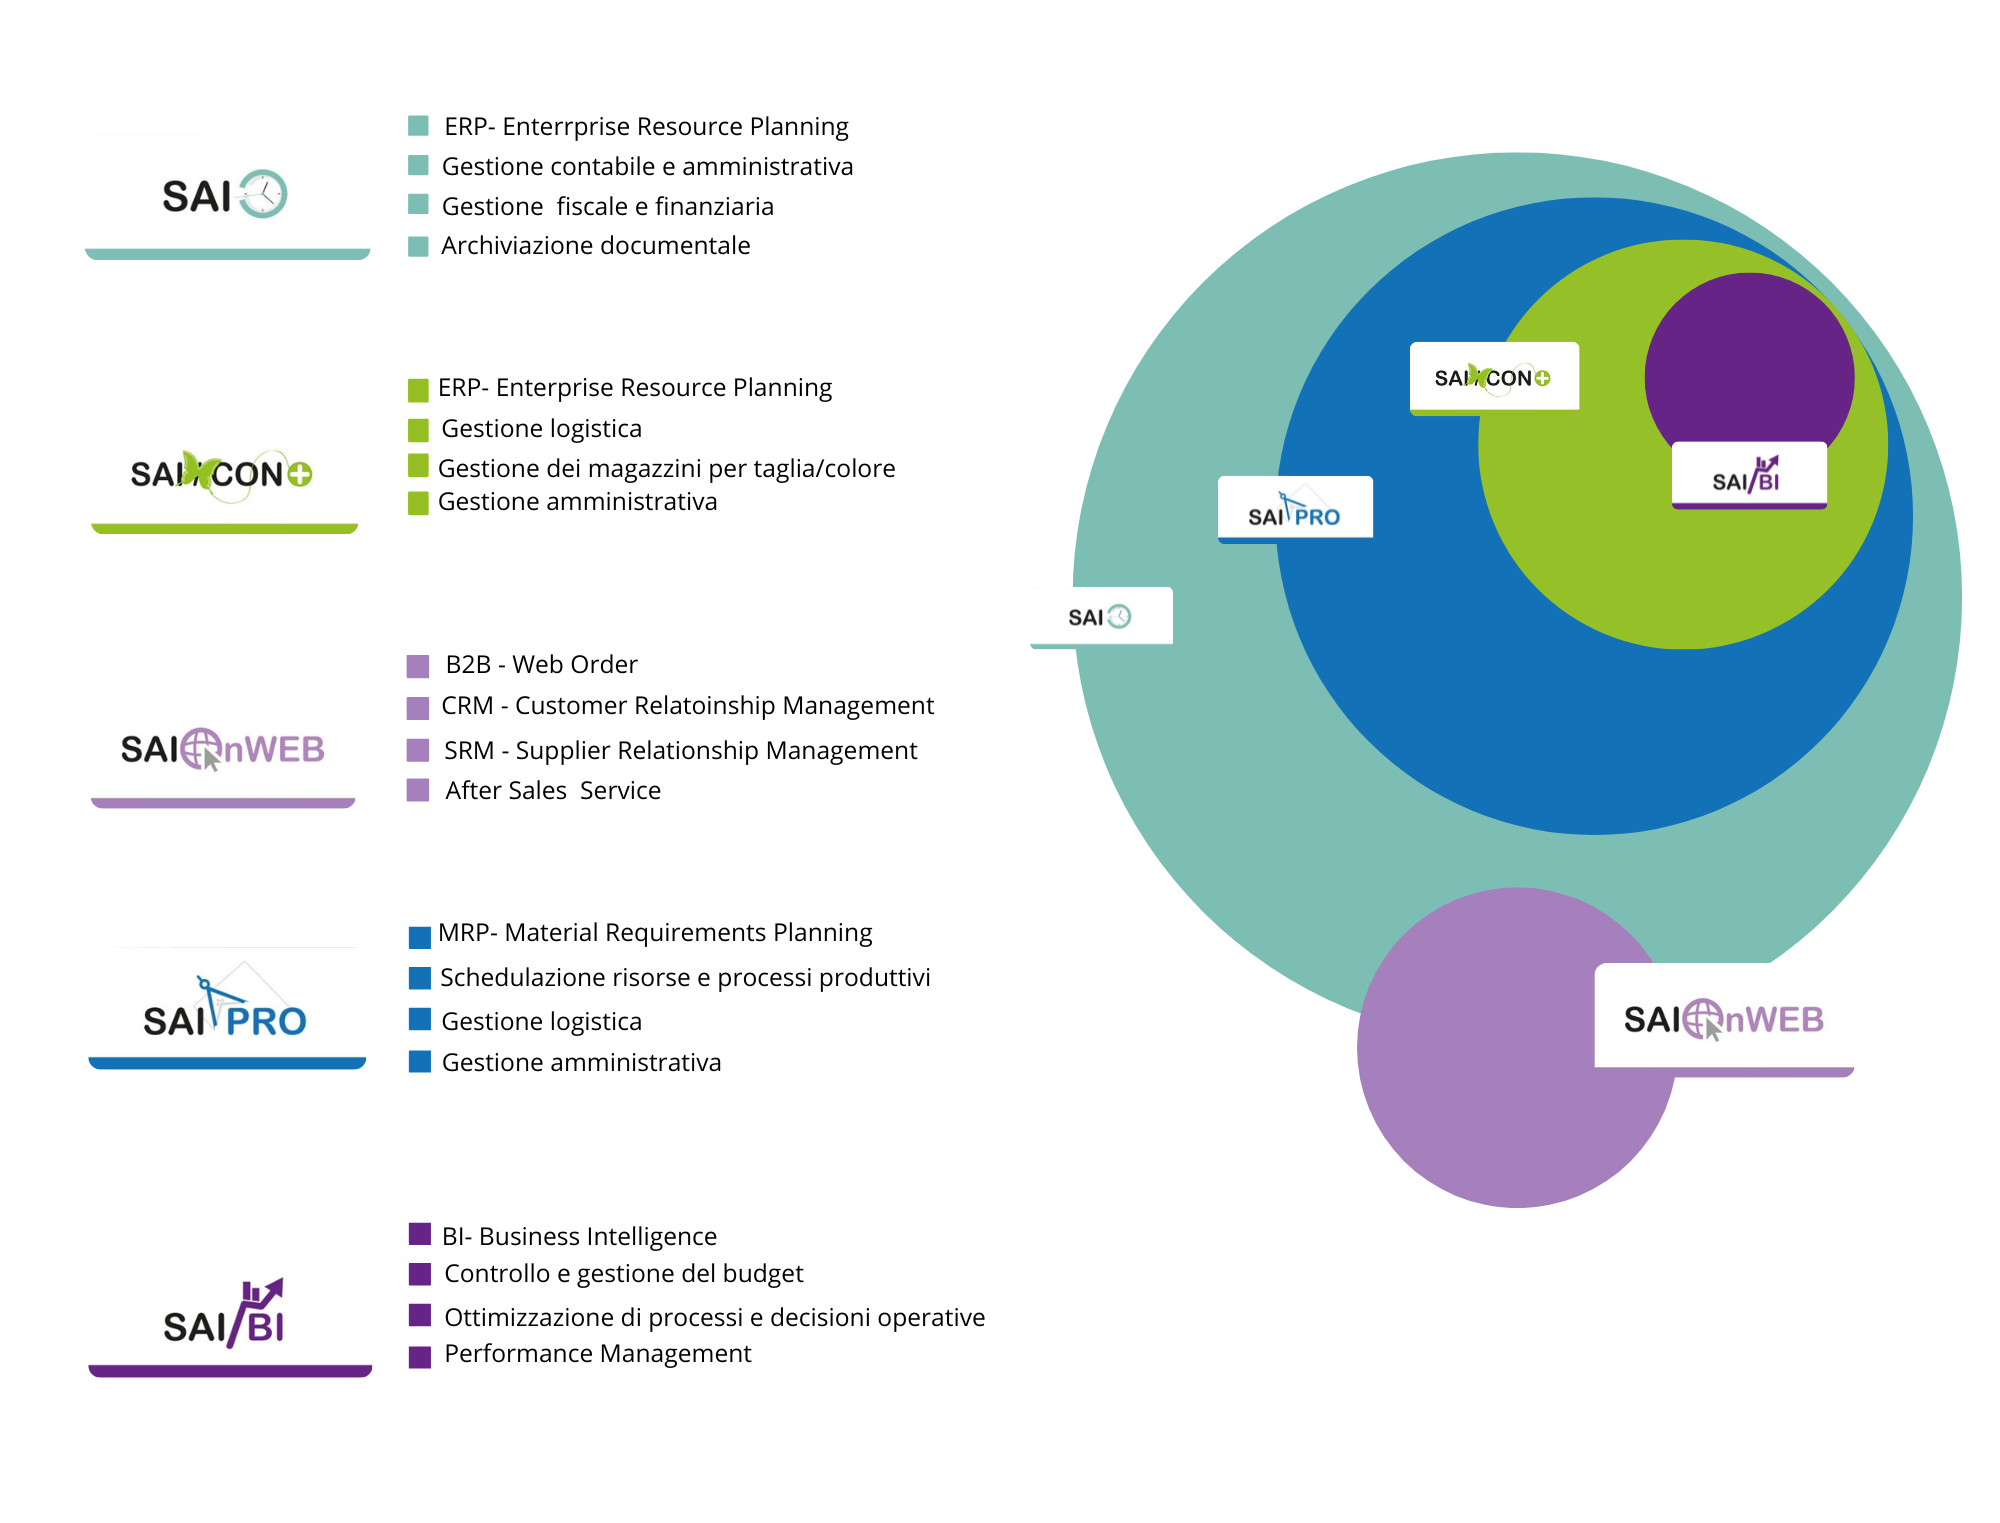
\includegraphics[width=0.9\linewidth]{BCS-Tessi/images/SOGEAProdotti.png}
        \caption[Prodotti di SogeaSoft S.r.l.]{Panoramica dei prodotti e servizi offerti da SogeaSoft S.r.l.}
        \label{fig:panoramica_prodotti}
    \end{figure}

    \noindent Come si può osservare in Figura 1.1, i principali prodotti di SogeaSoft S.r.l. sono strettamente interconnessi, il che si riflette nell’organizzazione dei \textit{team} all’interno dell’azienda. Sebbene esista una divisione indicativa basata sul tipo di prodotto sviluppato, i ruoli risultano essere sfumati e coprono più aree di competenza. 
    \noindent Le persone che lavorano su ciascun prodotto fanno riferimento a un \textit{Product Owner}, che può rappresentare più \textit{team} in base alle necessità.

    \noindent Durante il mio \textit{stage} ho avuto modo di interagire con: 
    \begin{itemize}
        \item \textbf{\textit{Product Owner}}: è la figura responsabile della definizione delle caratteristiche di un prodotto, della gestione delle priorità e della comunicazione con il \textit{team} di sviluppo, al fine di garantire che il prodotto finale soddisfi le esigenze degli utenti e gli obiettivi aziendali;
        
        \item \textbf{\textit{Team Leader}}: gestisce il \textit{team} di sviluppo. In SogeaSoft S.r.l. questa figura può coincidere con il \textit{Product Owner} e/o con il \textit{Scrum Master} (approfondito nella Sezione 1.4);
        \item \textbf{Sviluppatore}: si occupa di progettazione, sviluppo e \textit{testing} del \textit{software}. In base al grado di esperienza contribuisce anche all'analisi e all'assistenza ai clienti. 
    \end{itemize}


    \section{Prodotti di SogeaSoft S.r.l.}

    Il prodotto principale di SogeaSoft S.r.l. è un \textit{software} ERP denominato SAI. Costituisce la base per tutti gli altri prodotti sviluppati dall'azienda infatti fanno affidamento diretto su SAI. Nasce come \textit{software} per la gestione della contabilità, poi ampliato con il tempo e adattato a realtà manifatturiere; ciò ha portato la necessità di introdurre ulteriori funzionalità. 
    Nel contesto del mio stage ho potuto approfondire SAIOnWeb e SAIPro che sviluppano le seguenti funzionalità:
    \begin{itemize}
        \item \textbf{Material Requirements Planning (MRP)}: pianificazione per determinare i materiali necessari per la produzione, ottimizzando i tempi di approvvigionamento e garantendo la disponibilità delle componenti richieste;
        \item \textbf{Master Production Scheduling (MPS)}: piano di produzione dettagliato per garantire il rispetto degli impegni con i clienti, ottimizzando l’utilizzo delle risorse e coordinando la produzione con la domanda prevista;
        \item \textbf{Capacity Requirements Planning (CRP)}: analisi delle capacità produttive disponibili per verificare che siano adeguate a soddisfare i requisiti stabiliti dal piano di produzione;
        \item \textbf{Finite Capacity Scheduling (FCS)}: pianificazione dettagliata che considera i limiti effettivi delle risorse aziendali, ottimizzando l'allocazione e la sequenza delle attività produttive per massimizzare l'efficienza.       
    \end{itemize}
    
        \subsection{Target dell'azienda}
        SogeaSoft S.r.l. si rivolge principalmente alle Piccole e Medie Imprese (PMI), che spesso presentano la necessità di digitalizzare i propri processi aziendali, richiedendo al contempo un supporto tecnico affidabile e costante. 
        
        \vspace{0.2 em}
        
        \noindent Le PMI che rappresentano il \textit{target} principale dell’azienda operano prevalentemente nel settore manifatturiero e sono interessate a ottimizzare i propri flussi operativi. Questi includono la gestione e il monitoraggio delle \textit{performance} del personale, la regolazione e l’automazione dei processi logistici, e l’implementazione di soluzioni che migliorino la pianificazione, la produzione e il controllo dei costi.
        
    \section{Modello di sviluppo}
    SogeaSoft S.r.l. ha adottato un modello di sviluppo software basato sul \textit{$framework_G$} Scrum, una metodologia ispirata ai principi dello sviluppo \textit{Agile}. Questo approccio mira a ottimizzare il processo di lavoro rendendolo modulare, adattivo e in grado di rispondere rapidamente ai cambiamenti e alle necessità del cliente e alla complessità delle commesse.  

    \vspace{0.2 em}
    
    \noindent Alla base di Scrum vi è il concetto di \textit{User Story}, una descrizione ad alto livello delle funzionalità attese dal cliente o individuate dal \textit{Product Owner}. Le \textit{User Story}, raccolte nel \textit{Product Backlog}, costituiscono l'insieme di attività prioritarie che guidano lo sviluppo. Questo elenco viene costantemente aggiornato per riflettere nuove necessità o modificare le priorità.
    
    \vspace{0.2 em}
    \noindent Dopo essere state definite e raffinate, le \textit{User Story} guidano l'organizzazione e la pianificazione dello sviluppo, che avviene attraverso cicli iterativi chiamati \textit{Sprint}. Questo approccio consente di garantire un miglior controllo dei processi e un allineamento costante tra il \textit{team} di sviluppo e gli obiettivi aziendali. 

    \noindent Le principali cerimonie Scrum adottate sono visibili in un diagramma nella Figura 1.2, meglio descritte in seguito:
    \begin{itemize}
    
        \item \textbf{\textit{Sprint Planning}}: all'inizio di ogni \textit{Sprint}, il gruppo di lavoro partecipa a una sessione di pianificazione per selezionare gli elementi del \textit{backlog} da sviluppare. Gli obiettivi principali dello \textit{Sprint} vengono definiti insieme allo \textit{Sprint Goal}, che rappresenta il risultato principale atteso;

        \item \textbf{\textit{Daily Scrum}}: ogni giorno, il gruppo di sviluppo e lo \textit{Scrum Master} partecipano a un incontro breve, durante il quale si coordinano le attività e si identificano eventuali ostacoli. Questo garantisce un allineamento costante del gruppo verso gli obiettivi dello \textit{Sprint};

        \item \textbf{\textit{Sprint Review}}: alla fine dello \textit{Sprint}, gli incrementi di prodotto sviluppati vengono presentati. Sebbene in teoria questa fase preveda il coinvolgimento degli \textit{$stakeholder_G$}, nel caso di SogeaSoft S.r.l. il ruolo di collegamento con il cliente finale viene svolto dal \textit{Product Owner}, il quale raccoglie \textit{feedback} e li traduce in aggiornamenti per il \textit{backlog};  

        \item \textbf{\textit{Sprint Retrospective}}: questo momento di riflessione sul lavoro svolto è utilizzato dal gruppo di lavoro per identificare opportunità di miglioramento nel processo di sviluppo. Tuttavia, data la dimensione contenuta dei \textit{team} e la consolidata organizzazione del lavoro, questa cerimonia viene svolta solo quando necessario.  

        \item \textbf{Raffinamento del \textit{Backlog}}: un'altra attività fondamentale è quella del Raffinamento, che si tiene con cadenza regolare per preparare gli elementi del \textit{backlog} per i successivi \textit{Sprint}. Durante queste sessioni, il gruppo di lavoro collabora per suddividere le funzionalità più complesse in elementi più piccoli, chiarire i requisiti e definire criteri di accettazione. Questo processo garantisce che gli elementi siano chiari e pronti per essere inclusi nel prossimo \textit{Sprint Planning}. La responsabilità principale di questa attività ricade sul \textit{Product Owner}, con il supporto del \textit{team} di sviluppo.
        
    \end{itemize}
    
    \noindent In sintesi, il modello di sviluppo di SogeaSoft S.r.l. si basa su una gestione iterativa e collaborativa, che consente di rispondere, in un modo che si avvicina al modello \textit{Agile}, alle richieste dei clienti e di mantenere un flusso di lavoro efficace e focalizzato sugli obiettivi aziendali.

    \begin{figure}[H]
        \centering
        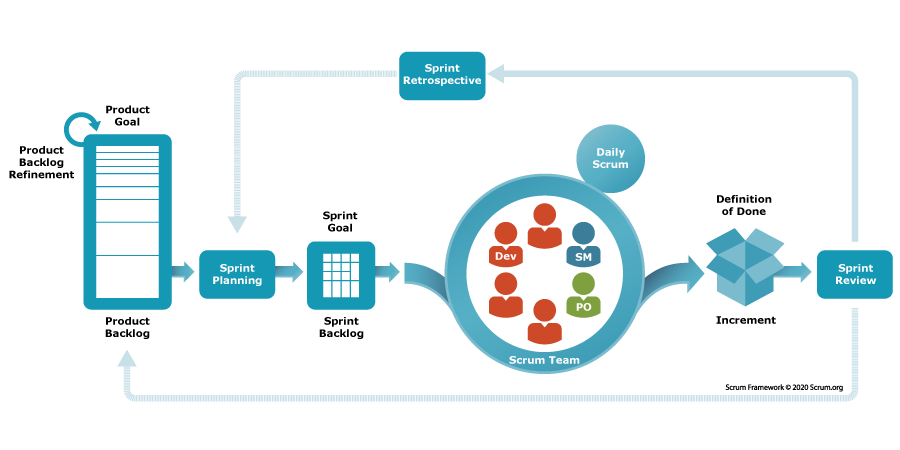
\includegraphics[width=0.8\linewidth]{BCS-Tessi/images/scrum_flow.png}
        \caption[Diagramma del modello Scrum]{Diagramma del flusso di lavoro del modello Scrum, basato sulla filosofia \textit{Agile}. \href{https://www.scrum.org/learning-series/what-is-scrum/}{Fonte: Documentazione Scrum} \textit{(ultimo accesso 3/03/2025)}}
        \label{fig:scrum_flow}
    \end{figure}
    
    \section{Organizzazione interna}
    SogeaSoft S.r.l. implementa i principi della norma \textbf{UNI EN ISO 9001:2015} per garantire un sistema di gestione della qualità dei prodotti efficace.\footnote{Fonte:\href{https://sogeasoft.com/p/iso9001}{ https://sogeasoft.com/p/iso9001} \textit{(ultimo accesso 3/03/2025)}}
    
    \vspace{0.2 em}
    \noindent Pur non essendo specificamente pensata per lo sviluppo \textit{software}, la norma trova applicazione nell’organizzazione grazie all’adozione di pratiche volte a standardizzare i processi e migliorare l’efficienza operativa. L'azienda basa la propria struttura sull'approccio per processi, suddividendo il lavoro in unità specializzate (come SAI, SAIPro e SAICon) e adottando metodologie \textit{Agile} per la pianificazione e gestione delle attività, ispirandosi allo standard ISO/IEC/IEEE 12207 (\textit{Systems and software engineering - Software life cycle processes}).

    \vspace{0.2 em}
    \noindent Anche i principi dell’approccio per processi e del metodo Plan-Do-Check-$Act_G$ ($PDCA_G$) sono applicati in tutte le fasi operative. Il PDCA si concretizza attraverso la pianificazione accurata delle attività (\textit{Plan}), la loro esecuzione (\textit{Do}), l’analisi dei risultati ottenuti (\textit{Check}) e l’implementazione di eventuali azioni correttive o migliorative (\textit{Act}).

    \vspace{0.2 em}
    \noindent Un esempio dell’applicazione del PDCA è riscontrabile nel modello di sviluppo Scrum, adottato da SogeaSoft S.r.l. per garantire iterazioni rapide e flessibili. Durante gli \textit{Sprint}, il \textit{backlog} viene pianificato e raffinato (\textit{Plan}), le attività vengono eseguite secondo le priorità stabilite (\textit{Do}), e i risultati sono presentati e analizzati attraverso la \textit{Sprint Review} e la \textit{Retrospective} (\textit{Check}). Eventuali miglioramenti vengono quindi incorporati negli \textit{Sprint} successivi (\textit{Act}).

    \vspace{0.2 em}
    \noindent La Figura 1.3 mostra il certificato UNI EN ISO 9001:2015 ottenuto dall’azienda, che conferma l’impegno di SogeaSoft S.r.l. nel mantenere elevati standard di qualità nei propri processi.

    \begin{figure}[H]
        \centering
        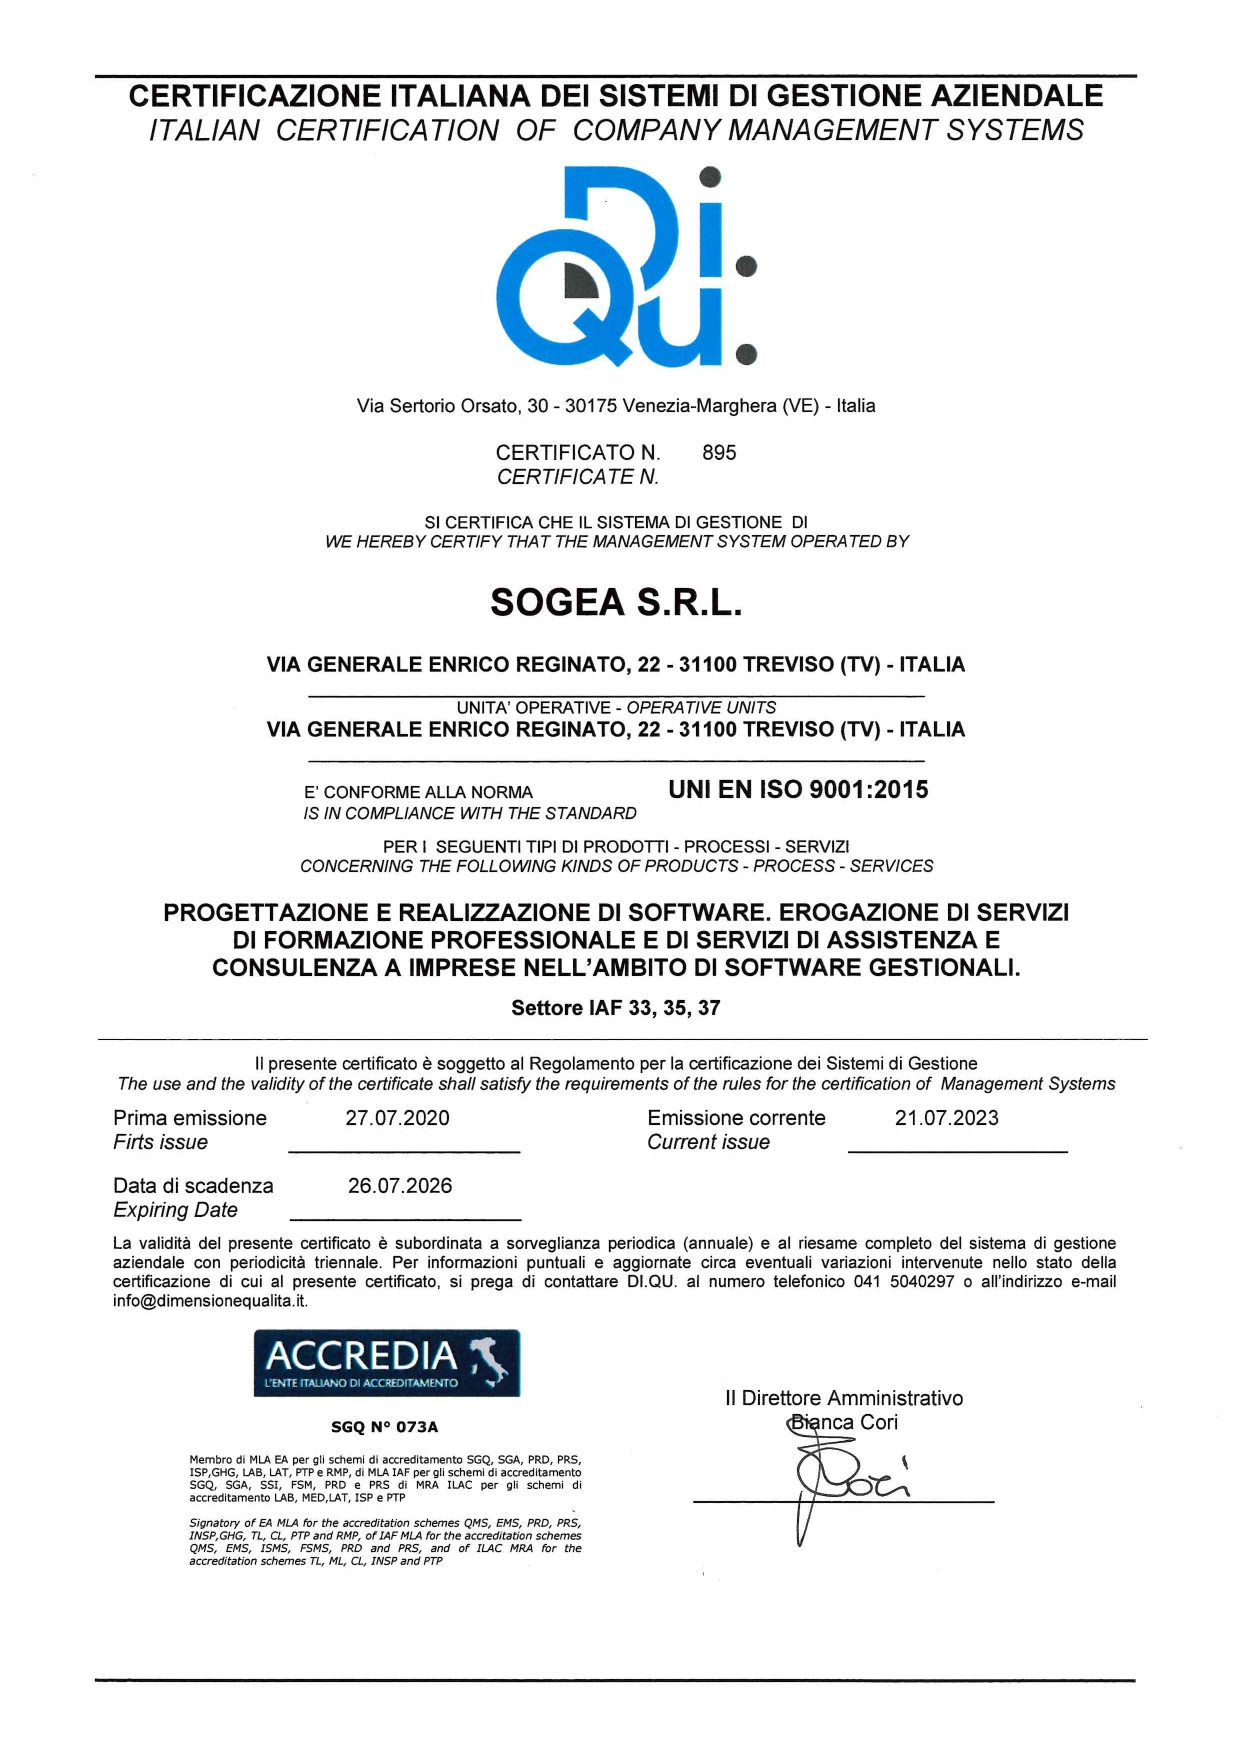
\includegraphics[width=0.5\linewidth]{BCS-Tessi/images/CertificatoSogea.jpg}
        \caption[Certificazione ISO di SogeaSoft S.r.l.]{Certificazione ISO ottenuta da SogeaSoft S.r.l. \href{https://sogeasoft.com/p/iso9001}{Fonte: Documentazione pubblica di SogeaSoft S.r.l.}
        \textit{(ultimo accesso 26/02/2025)}}
        \label{fig:certificazione-iso}
    \end{figure}

    \noindent Nelle sezioni successive analizzerò alcuni aspetti fondamentali della gestione del ciclo di vita del \textit{software} all'interno di SogeaSoft S.r.l., con particolare attenzione ai processi di supporto che garantiscono l'efficienza e la qualità dello sviluppo. In particolare approfondirò i processi di cui ho avuto esperienza diretta, come la \textbf{Gestione della configurazione} (Sezione 1.5.1), essenziale per tracciare e controllare le modifiche al codice e alle risorse del sistema; la \textbf{Gestione dell’informazione} (Sezione 1.5.2), che disciplina la documentazione e la condivisione delle conoscenze all'interno dell'azienda; e la \textbf{Gestione delle risorse umane} (Sezione 1.5.3), fondamentale per il coordinamento dei \textit{team} e la formazione del personale. 
    
    
        \subsection{Gestione della configurazione}
        Lo scopo del processo di Gestione della configurazione è stabilire e mantenere l'integrità di tutti gli \textit{output} identificati di un progetto o processo e renderli disponibili alle parti interessate.\footnote{ISO/IEC/IEEE 12207:2008, Configuration Management process, par. 6.3.5.}

        \vspace{0.2 em}
        \noindent Nello specifico, un sistema di controllo è importante nell'evoluzione delle funzionalità del \textit{software}, del codice e della documentazione associata perché essi costituiscono gli \textit{output} in questione. Ciò permette di mantenere traccia delle modifiche e garantire che ogni versione sia controllata, riproducibile e coerente con i requisiti stabiliti, facilitando così la gestione delle evoluzioni del \textit{software} e la collaborazione tra i membri del \textit{team}. 
        
        \vspace{0.2 em}
        \noindent In SogeaSoft S.r.l. il controllo delle modifiche al codice avviene attraverso un \textit{Version Control $System_G$} ($VCS_G$), che traccia l’evoluzione del \textit{software} in modo strutturato. Le versioni del codice vengono archiviate all’interno di \textit{$repository_G$}, strutture dati appositamente organizzate per gestire i cambiamenti. 
        \noindent Queste \textit{repository} si basano su tre principali tipologie di \textit{$branch_G$}, ossia rami di sviluppo:  
        \begin{itemize}
            \item \textbf{master}: è il \textit{branch} principale e stabile, contenente il codice pronto per la produzione. Ogni versione ufficiale del \textit{software} viene rilasciata a partire da questo \textit{branch}; 
            \item \textbf{develop}: è il \textit{branch} destinato allo sviluppo continuo, in cui confluiscono le nuove funzionalità e le modifiche prima di essere integrate nel \textit{master}. Rappresenta una versione stabile ma non definitiva del \textit{software}; 
            \item \textbf{release}: sono \textit{branch} temporanei creati a partire dal \textit{develop} per preparare un rilascio specifico. 
        \end{itemize}

        \noindent La documentazione viene gestita all'interno di un'area dedicata dell'ambiente di sviluppo adottato (Sezione 1.5.2) da SogeaSoft S.r.l., denominata Wiki. Questo sistema organizza le informazioni in base ad argomenti, capitoli e finalità d'uso, garantendo una struttura relativamente chiara. Inoltre, ogni modifica è accompagnata da un \textit{timestamp} e dall'identificativo dell'autore, permettendo un tracciamento preciso delle revisioni. 
        
        \subsection{Gestione dell’informazione}

        Lo scopo del Processo di Gestione delle Informazioni è garantire alle parti designate l’accesso a informazioni pertinenti, tempestive, complete e valide durante e, ove opportuno, dopo il ciclo di vita del sistema.\footnote{ISO/IEC/IEEE 12207:2008, Information Management process, par. 6.3.6.}

        \vspace{0.2 em}
        \noindent SogeaSoft S.r.l. impiega la piattaforma Microsoft Azure sia per la scrittura del codice sia per la gestione della documentazione aziendale. Questo strumento collaborativo facilita l'integrazione con diversi sistemi di supporto ai processi di Gestione della Configurazione, Progettazione, Implementazione e Manutenzione. In particolare, per la documentazione, SogeaSoft S.r.l. utilizza le Wiki (Figura 1.4), che consentono di organizzare e strutturare le informazioni in modo sistematico.  

        \begin{figure}[H]
            \centering
            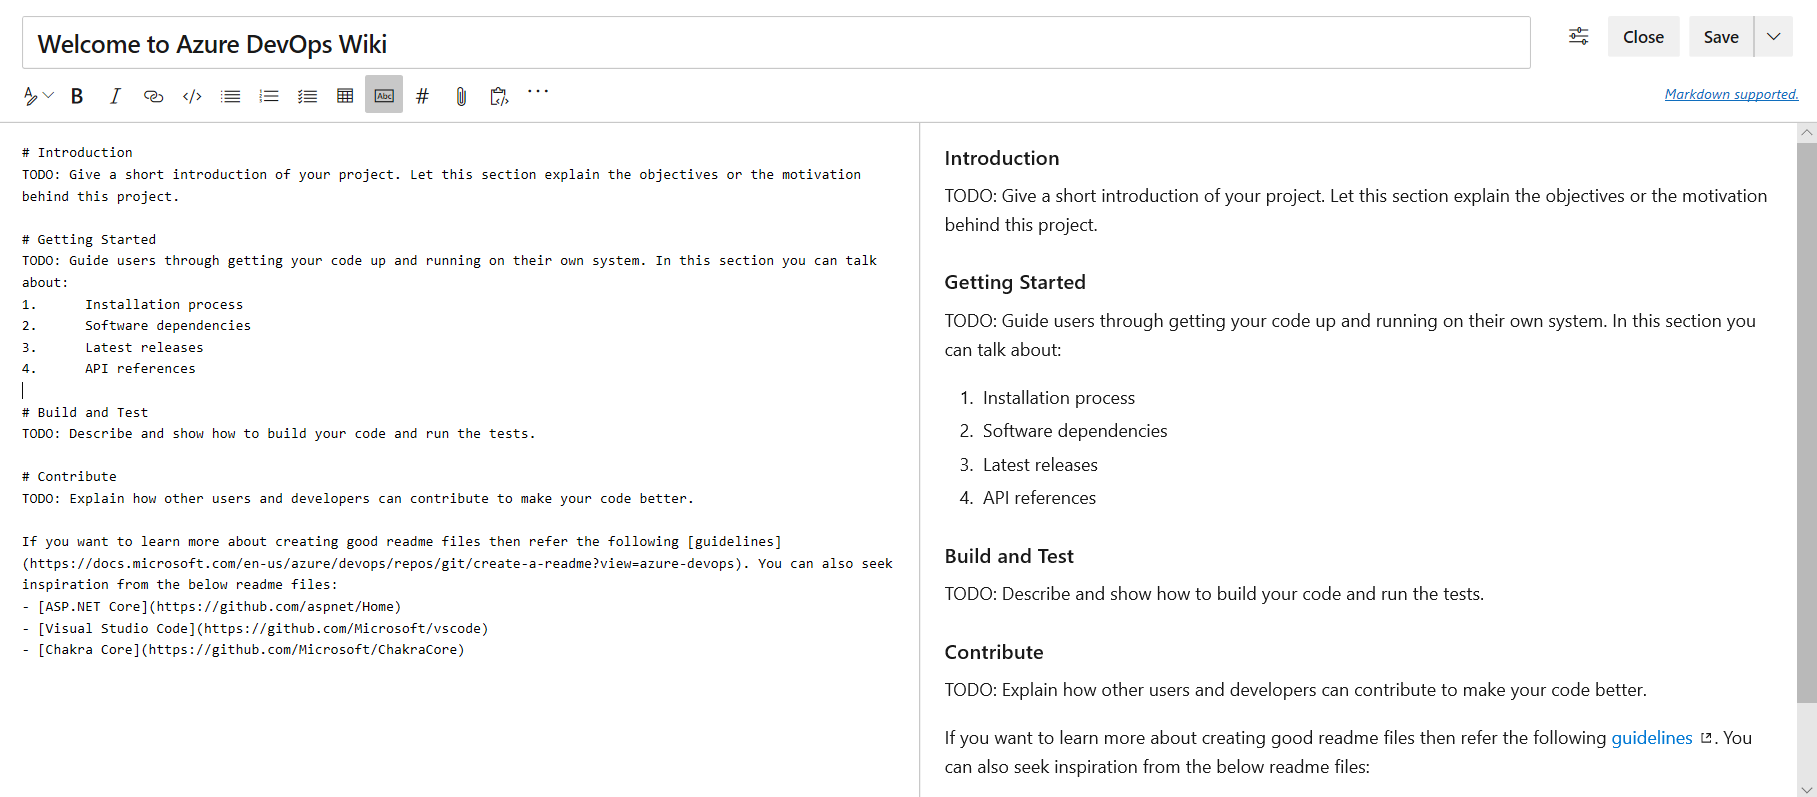
\includegraphics[width=0.9\linewidth]{BCS-Tessi/images/Wiki_Azure.png}
            \caption[Microsoft Azure, Wiki]{Esempio di Wiki in Microsoft Azure. \href{https://learn.microsoft.com/it-it/azure/devops/project/wiki/add-edit-wiki?view=azure-devops&tabs=browser}{Fonte: Documentazione Microsoft Azure} \textit{(ultimo accesso 1/03/2025)}}
            \label{fig:Wiki}
        \end{figure}
        
        \noindent Durante il mio \textit{stage}, ho osservato come, data l’interoperabilità del \textit{software} aziendale, risulti fondamentale che la documentazione associata sia formalmente strutturata in documenti accessibili a tutti i membri dei \textit{team}. Tale documentazione segue una gerarchia ben definita, comprendente la registrazione di incontri, requisiti, analisi e scelte progettuali, tutte adeguatamente descritte e motivate.  

        \vspace{0.2 em}
        \noindent Tuttavia, questo approccio non è sempre stato adottato in maniera sistematica. Nelle versioni più datate del \textit{software}, la documentazione risultava spesso incompleta o assente, costringendo gli sviluppatori a ricorrere al \textit{reverse engineering} per comprendere il funzionamento del codice. Questa criticità ha generato una forte dipendenza dalle conoscenze dei singoli sviluppatori coinvolti nel processo iniziale, rendendo più complesso l’apporto di modifiche e aggiornamenti successivi.  

        \vspace{0.2 em}
        \noindent Da qui deriva la necessità di SogeaSoft S.r.l. di abbandonare gradualmente il vecchio sistema in favore di un nuovo sistema più documentato, decentralizzato e flessibile. 
        
        \subsection{Processi di formazione}
        
        La gestione delle risorse umane rappresenta un elemento fondamentale per garantire all'organizzazione le competenze necessarie in linea con le esigenze aziendali. Questo processo assicura la disponibilità di personale qualificato e con esperienza, in grado di svolgere le attività del ciclo di vita del \textit{software} e contribuire al raggiungimento degli obiettivi aziendali, di progetto e del cliente.\footnote{ISO/IEC/IEEE 12207:2008, Human Resource Management process, par. 6.3.4.}

        \vspace{0.2 em}
        \noindent Durante il mio \textit{stage} ho avuto modo di analizzare le modalità adottate da SogeaSoft S.r.l. per la formazione dei propri dipendenti. L'azienda implementa un approccio articolato, combinando diverse metodologie formative per garantire un apprendimento efficace e continuo. In particolare, le strategie impiegate comprendono:

        \begin{enumerate}
        \item \textbf{Lezioni in presenza}: nel caso in cui l’azienda intenda introdurre nuove tecnologie o apportare modifiche significative ai \textit{software} in uso, vengono organizzati corsi di formazione condotti da esperti del settore;

        \item \textbf{Autoapprendimento}: successivamente alle lezioni frontali, i dipendenti sono incoraggiati a integrare e approfondire autonomamente le conoscenze acquisite. Tale processo avviene attraverso la consultazione di libri tecnici, la visione di videolezioni su piattaforme online gratuite e l’analisi di progetti preesistenti affini;

        \item \textbf{Peer programming}: questa pratica collaborativa prevede il coinvolgimento di due o più programmatori nella scrittura del codice, promuovendo la condivisione di competenze e il miglioramento della qualità del \textit{software}.
        \end{enumerate}
        
        \noindent Nel corso del mio stage ho applicato prevalentemente le metodologie di \textbf{autoapprendimento} e \textit{\textbf{peer programming}}. Come si può osservare in Figura 1.5, nelle prime settimane la ricerca autonoma di informazioni e il confronto diretto con colleghi più esperti hanno occupato gran parte della mia giornata lavorativa. Tuttavia, con il progressivo consolidamento delle competenze acquisite, dopo circa dieci giorni lavorativi ho potuto ridurre significativamente il tempo dedicato allo studio individuale,  limitando il ricorso al \textit{peer programming} ai soli casi in cui si presentassero difficoltà specifiche nello sviluppo del \textit{software}.

        \begin{figure} [H]
            \centering
            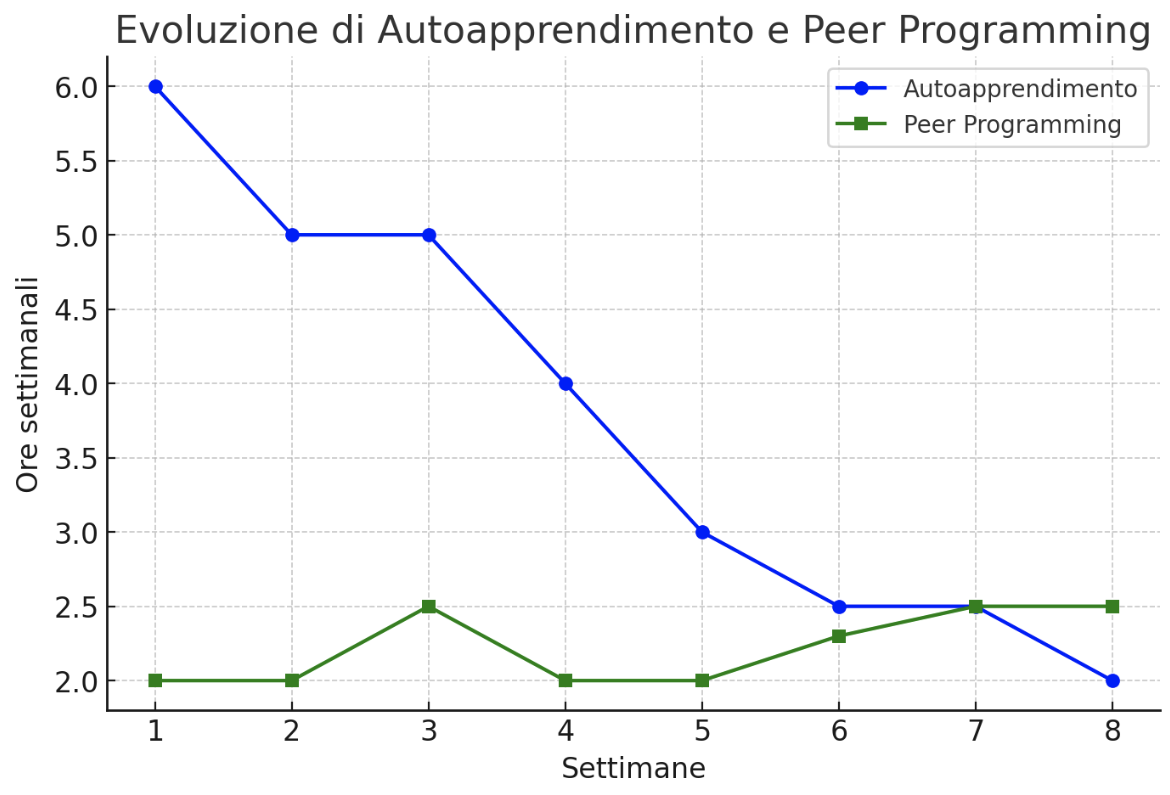
\includegraphics[width=0.8\linewidth]{BCS-Tessi/images/Rendicontazione_ore.png}
            \caption[Rendicontazione ore dedicate alla formazione]{Rendicontazione ore dedicate ai processi di formazione durante il mio \textit{stage}}
            \label{fig:Ore-formazione}
        \end{figure}
        

    \section{Ciclo di vita di un progetto software}
    Il ciclo di vita di un progetto \textit{software} rappresenta l’insieme delle fasi attraverso cui un sistema viene ideato, sviluppato, verificato e mantenuto nel tempo.\footnote{I. Sommerville, Software Engineering, 10ª ed., Boston, MA, USA: Pearson, 2015.} Nell’ambito dello sviluppo \textit{Agile}, tale processo assume una natura iterativa e incrementale, consentendo una maggiore flessibilità nell’adattamento ai requisiti in evoluzione e nell’ottimizzazione continua del prodotto.

    \vspace{0.2 em}
    \noindent Lo standard ISO/IEC/IEEE 12207 fornisce un quadro di riferimento formale per la gestione del ciclo di vita del \textit{software}, delineando attività strutturate per la pianificazione, lo sviluppo e la manutenzione. Le sezioni successive approfondiranno le principali fasi del ciclo di vita del software nel contesto aziendale di SogeaSoft S.r.l., con particolare riferimento all’esperienza maturata durante il mio \textit{stage}.
        \subsection{Analisi preliminare e raccolta dei requisiti}
        L’analisi dei bisogni degli \textit{stakeholder} e la raccolta dei requisiti rappresentano fasi fondamentali nel ciclo di vita di un progetto \textit{software}, poiché definiscono le basi su cui verrà sviluppato il sistema.\footnote{ISO/IEC/IEEE 12207:2008, Stakeholder Requirements Definition Process, par. 6.4.1.} Secondo lo standard ISO/IEC/IEEE 12207, tali attività rientrano nel processo di gestione dei requisiti e hanno l’obiettivo di identificare, documentare e validare le esigenze delle parti interessate, garantendo che il \textit{software} finale sia allineato alle aspettative degli utenti. 

        \vspace{0.2 em}
        \noindent Gli \textit{stakeholder} di un progetto \textit{software} possono includere clienti, utenti finali, \textit{team} di sviluppo, responsabili di prodotto e altre figure coinvolte nel ciclo di vita del sistema. L’analisi dei bisogni si concentra sull’identificazione delle problematiche esistenti, sulle necessità operative e sugli obiettivi strategici che il \textit{software} deve supportare. Tale attività si avvale di tecniche come interviste, \textit{workshop}, questionari e l’osservazione diretta dei processi aziendali.

        \vspace{0.2 em}
        \noindent Nel contesto dello sviluppo \textit{Agile}, questa fase è dinamica e continua: i bisogni vengono esplorati progressivamente, attraverso interazioni frequenti con gli \textit{stakeholder}. Per favorire la collaborazione costante tra le parti, il \textit{Product Owner} agisce come intermediario tra il \textit{team} di sviluppo e le parti interessate, assicurando che le priorità del prodotto riflettano i reali bisogni dell’azienda.

        \vspace{0.2 em}
        \noindent Una volta analizzati i bisogni, si procede con la definizione e la formalizzazione dei requisiti, ovvero le specifiche funzionali e non funzionali che il \textit{software} dovrà soddisfare. I requisiti funzionali descrivono le capacità e le operazioni del sistema, mentre quelli non funzionali riguardano aspetti come prestazioni, sicurezza, usabilità e scalabilità.\footnote{ISO/IEC/IEEE 12207:2008, System Requirements Analysis Process, par 6.4.2.}

        \vspace{0.2 em}
        \noindent Nello specifico SogeaSoft S.r.l. applica il concetto di \textit{$Domain-Driven Design_G$} ($DDD_G$), un approccio che permea l’intero ciclo di vita dello sviluppo \textit{software}, contribuendo a modellare il dominio in maniera coerente e a garantire che il sistema sviluppato risponda in modo preciso e scalabile alle esigenze precedentemente identificate.\footnote{E. Evans, Domain-Driven Design: Tackling Complexity in the Heart of Software, Addison-Wesley, 2003} Una visione d'insieme dell'approccio si può osservare nella Figura 1.8.
        Nel contesto dell'analisi dei requisiti l'introduzione di DDD comporta diversi passaggi chiave (visualizzabili anche nella Figura 1.6):

        \begin{itemize}
        \item \textbf{Collaborazione con gli esperti del dominio} (\textit{\textbf{domain} $\textbf{experts}_G$}): l’elemento distintivo di DDD è il coinvolgimento continuo degli esperti del dominio, che sono coloro che possiedono una conoscenza approfondita del contesto in cui il sistema deve operare. Durante l'analisi dei requisiti, il \textit{team} di sviluppo e gli esperti di dominio lavorano a stretto contatto per assicurarsi che i requisiti non siano solo funzionali, ma riflettano una comprensione profonda delle dinamiche del \textit{business}.

        \item \textbf{Creazione di un linguaggio comune} (\textit{\textbf{Ubiquitous} $\textbf{Language}_G$}): uno degli aspetti centrali di DDD è l’adozione di un linguaggio comune, che consente a tutte le parti coinvolte nel progetto (sia tecniche che non) di discutere in modo chiaro e preciso i concetti chiave del dominio. Questo linguaggio deve essere utilizzato sin dalla fase di analisi dei requisiti per evitare ambiguità e garantire che tutti i requisiti siano ben definiti.

        \item \textbf{Definizione di \textit{Bounded $\textbf{Context}_G$}}: un altro concetto fondamentale di DDD è la divisione del dominio in \textit{Bounded Contexts}. Durante l'analisi dei requisiti, i \textit{team} identificano e definiscono questi contesti limitati, ciascuno con il proprio modello di dominio, che può evolvere in modo indipendente dagli altri. Questo aiuta a evitare conflitti tra requisiti di diverse parti del sistema e facilita la gestione della complessità, permettendo di concentrarsi su una parte specifica del dominio alla volta.
        \end{itemize}

        \begin{figure} [H]
            \centering
            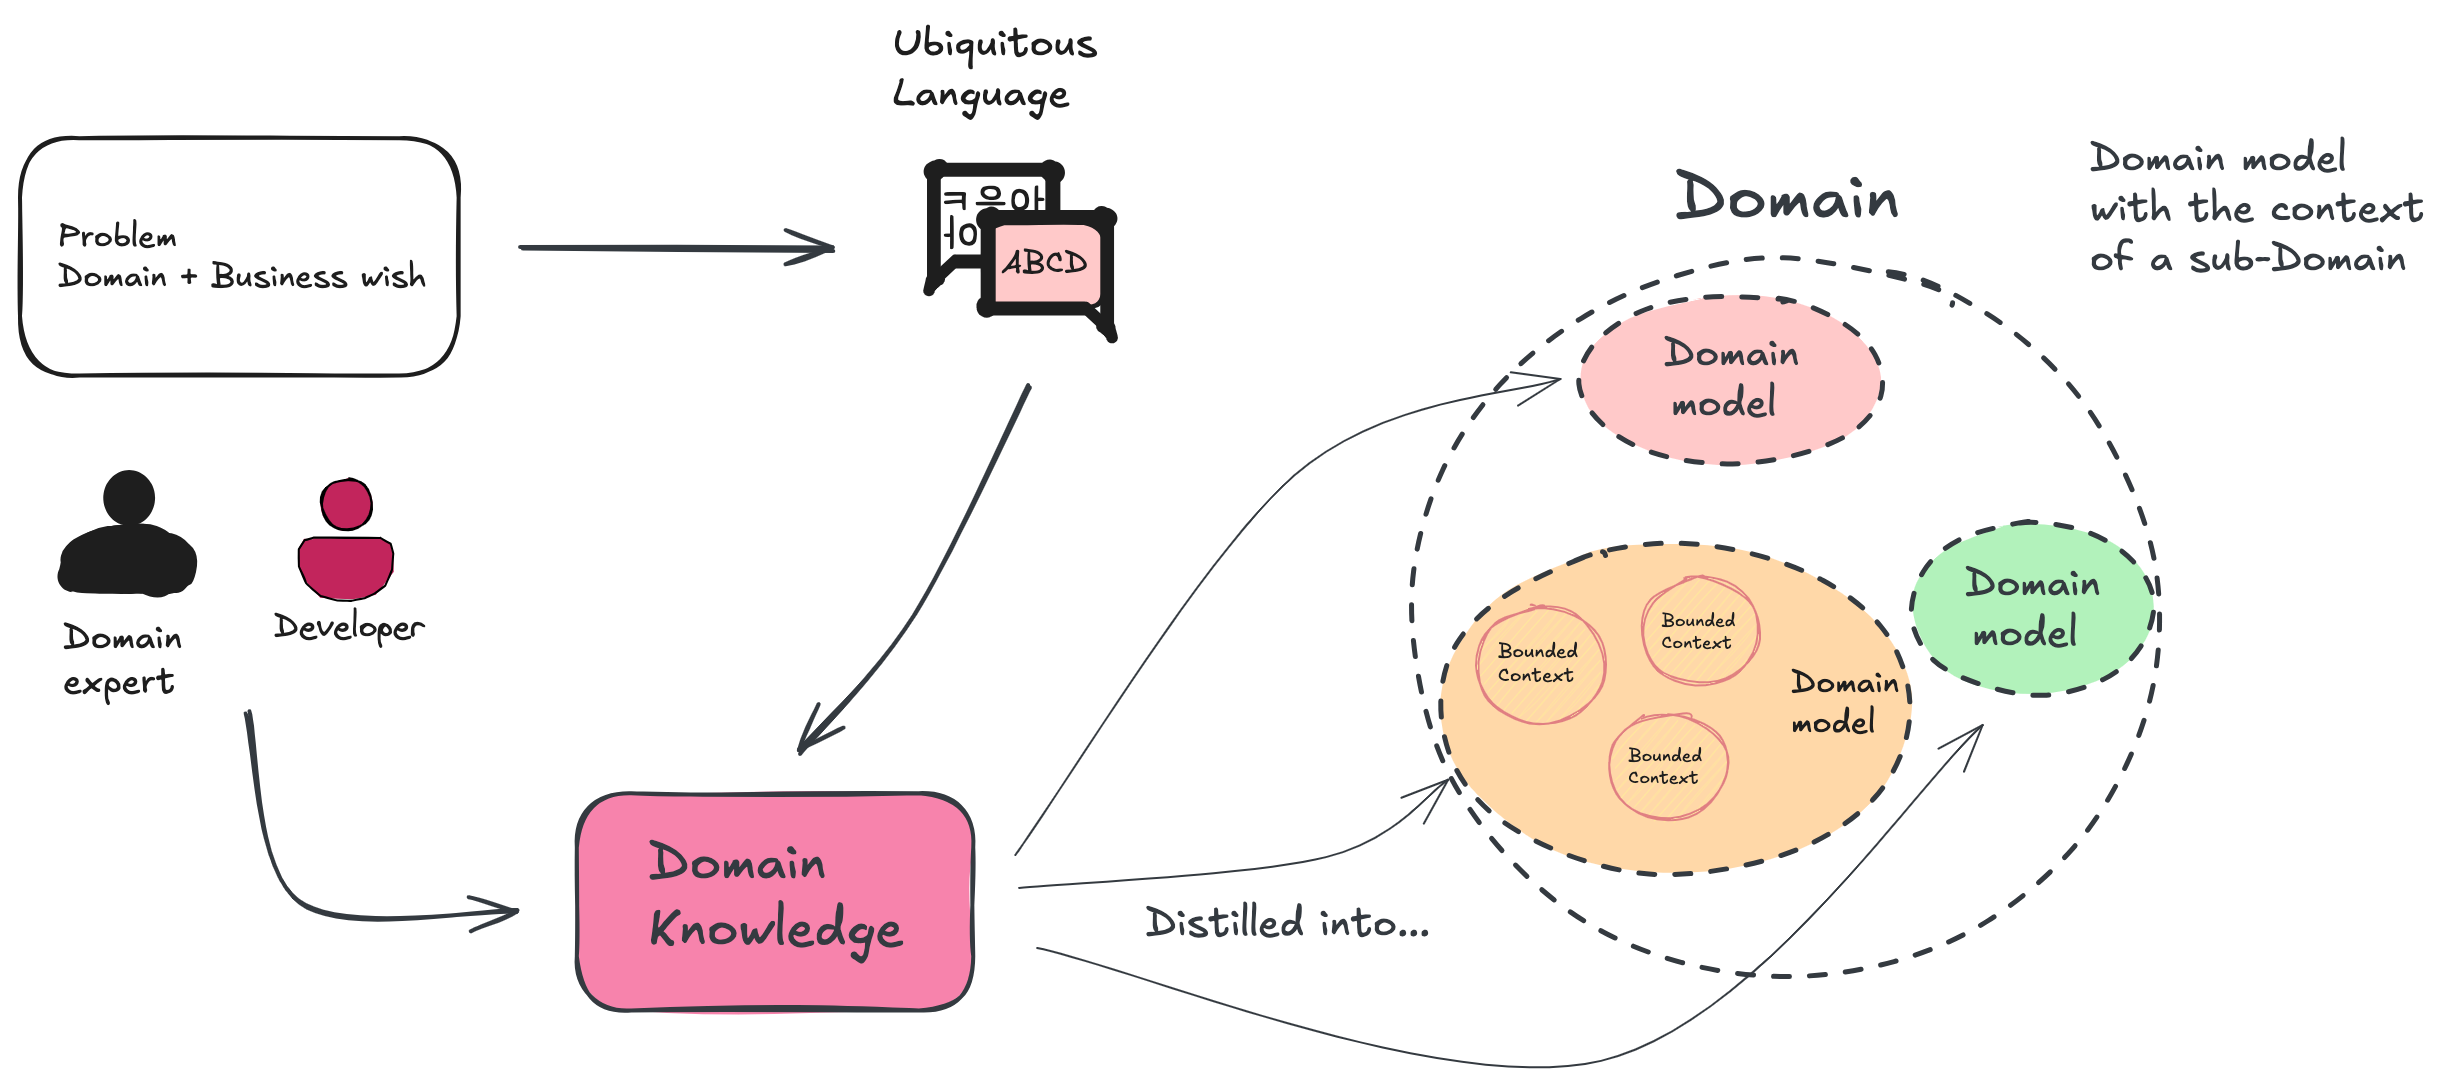
\includegraphics[width=0.9\linewidth]{BCS-Tessi/images/DDD_AR.png}
            \caption[Schema Analisi dei Requisiti nel contesto DDD]{Visualizzazione del processo di Analisi dei Requisiti nel contesto DDD.}
            \label{fig:AR-DDD}
        \end{figure}

        \noindent In conclusione, l’integrazione del \textit{Domain-Driven Design} nell’analisi dei requisiti consente di sviluppare un modello del dominio solido e coerente, facilitando la comunicazione tra gli \textit{stakeholder} e il \textit{team} di sviluppo. L’adozione di un linguaggio comune e la definizione di \textit{Bounded Contexts} contribuiscono a ridurre le ambiguità e a migliorare l’allineamento tra le esigenze di business e le soluzioni \textit{software}.
        
        \subsection{Progettazione}
        Il processo di Progettazione \textit{software} rappresenta una fase centrale del ciclo di vita dello sviluppo, in cui vengono definite l'architettura, i componenti e le interazioni del sistema al fine di garantire un’implementazione efficiente e conforme ai requisiti precedentemente raccolti.\footnote{ISO/IEC/IEEE 12207:2008, System Architectural Design Process, par 6.4.3.} 

        \vspace{0.2 em}
        \noindent Come previsto da Scrum (Sezione 1.4), io e il \textit{team} di sviluppo abbiamo iterato le attività di analisi e progettazione, con l'obiettivo di raggiungere delle soluzioni che potessero soddisfare i bisogni del cliente.

        \vspace{0.2 em}
        \noindent In particolare, con l'approccio del \textit{Domain-Driven Design}, introdotto nella Sezione 1.6.1, abbiamo attuato le seguenti attività visibili anche in Figura 1.7:
        \begin{itemize}
            \item \textbf{Modellazione del dominio}: dopo aver raccolto i requisiti, la fase di progettazione è dove l'approccio DDD inizia a entrare in gioco più attivamente. Utilizzando il linguaggio comune e i concetti emersi durante l'analisi dei requisiti, io e il \textit{team} di sviluppo abbiamo abbiamo costruito un modello di dominio dettagliato. In questa fase abbiamo definito gli $aggregati_G$, le $entità_G$, i \textit{value $objects_G$} e le funzioni di dominio, tutti elementi di progettazione nel contesto DDD. 
            \item \textbf{Definizione degli eventuali $\textbf{microservizi}_G$}: data la natura del progetto di \textit{stage}, l'approccio DDD ci ha aiutati a individuare delle unità autonome grazie ai \textit{Bounded Contexts} precedemente indentificati. Questo processo verrà approfondito nella Sezione 2.
            \item \textbf{Individuazione di $\textbf{pattern}_G$ di progettazione}: durante la fase di progettazione, l’approccio DDD impiega diversi \textit{pattern} architetturali e di \textit{design} per affrontare le problematiche comuni che emergono nella costruzione di sistemi complessi.\footnote{E. Evans, Domain-Driven Design: Tackling Complexity in the Heart of Software, Addison-Wesley, 2003} Questi \textit{pattern} ci hanno permesso di trovare modi per gestire in modo efficace la comunicazione tra le varie parti del sistema per poi poterle implementare nella fase successiva.
        \end{itemize}

        \begin{figure}
            \centering
            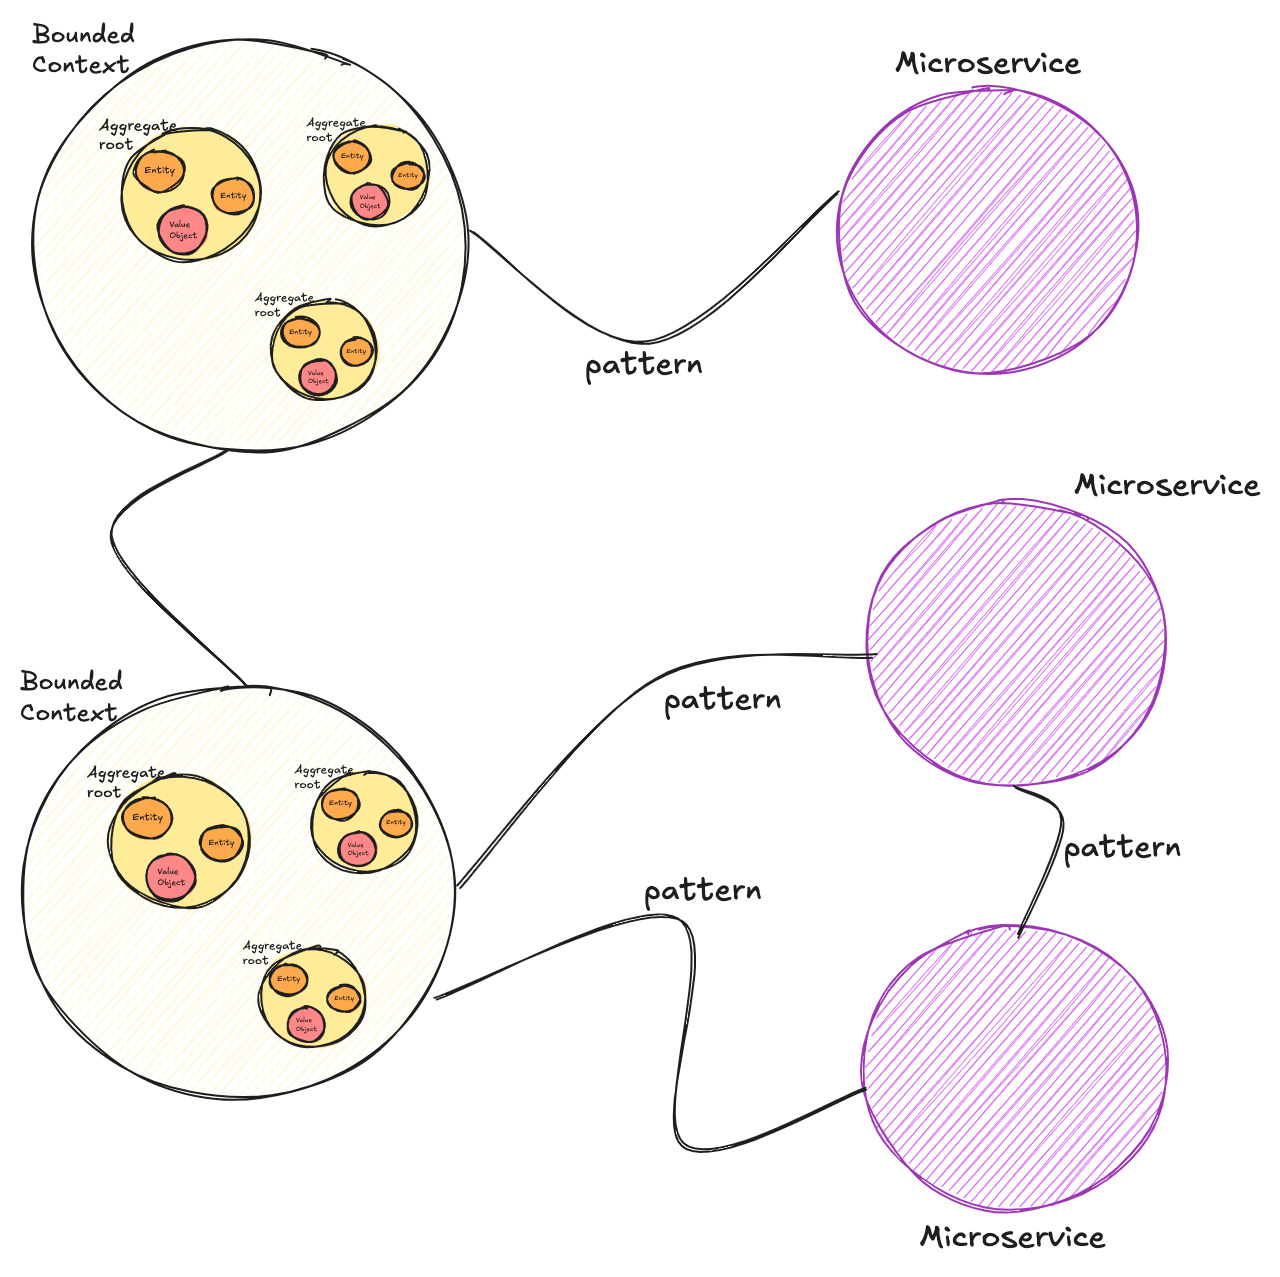
\includegraphics[width=0.5\linewidth]{BCS-Tessi/images/Progettazione_DDD.png}
            \caption{Schema dell'attività di Progettazione nel contesto DDD}
            \label{fig:progettazione-DDD}
        \end{figure}
        
        \subsection{Implementazione}
        
        L'attività di Implementazione costituisce una fase essenziale nel ciclo di vita del \textit{software}, in cui la soluzione progettata viene tradotta in codice eseguibile, rendendola concretamente fruibile dagli utenti finali. Secondo lo standard ISO/IEC/IEEE 12207, l'implementazione rientra nei processi primari di sviluppo e comprende la scrittura, la verifica e l'integrazione del codice, garantendo che il prodotto software soddisfi i requisiti definiti nelle fasi precedenti.\footnote{ISO/IEC/IEEE 12207:2008, Software Implementation Processes, par.7.1.} 

        \vspace{0.2 em}
        \noindent Per la gestione e il monitoraggio delle attività di codifica, l'azienda SogeaSoft S.r.l. utilizza Microsoft Azure, una piattaforma che integra un \textit{Issue Tracking $System_G$} ($ITS_G$). Questo strumento consente di gestire e tracciare le attività di sviluppo, offrendo una visione olistica del progetto sia dal punto di vista gestionale che implementativo.

        \vspace{0.2 em}
        \noindent Come è possibile osservare nella Figura 1.8, nel contesto del \textit{Domain-Driven Design} (DDD) l’implementazione segue principi mirati a garantire la coerenza tra il modello concettuale del dominio e la struttura del codice. In particolare, la fase di sviluppo prevede la codifica del modello di dominio.
        Quest'ultimo, elaborato durante la fase di Progettazione (Sezione 1.6.2), viene tradotto in codice attraverso l'implementazione delle componenti individuate nella fase precedente. Tali componenti vengono strutturate in modo da rispettare le regole di business definite in precedenza, utilizzando il linguaggio comune (\textit{Ubiquitous Language}) condiviso tra gli \textit{stakeholder} per assicurare consistenza semantica.\footnote{E. Evans, Domain-Driven Design: Tackling Complexity in the Heart of Software, Addison-Wesley, 2003}

        \begin{figure}
            \centering
            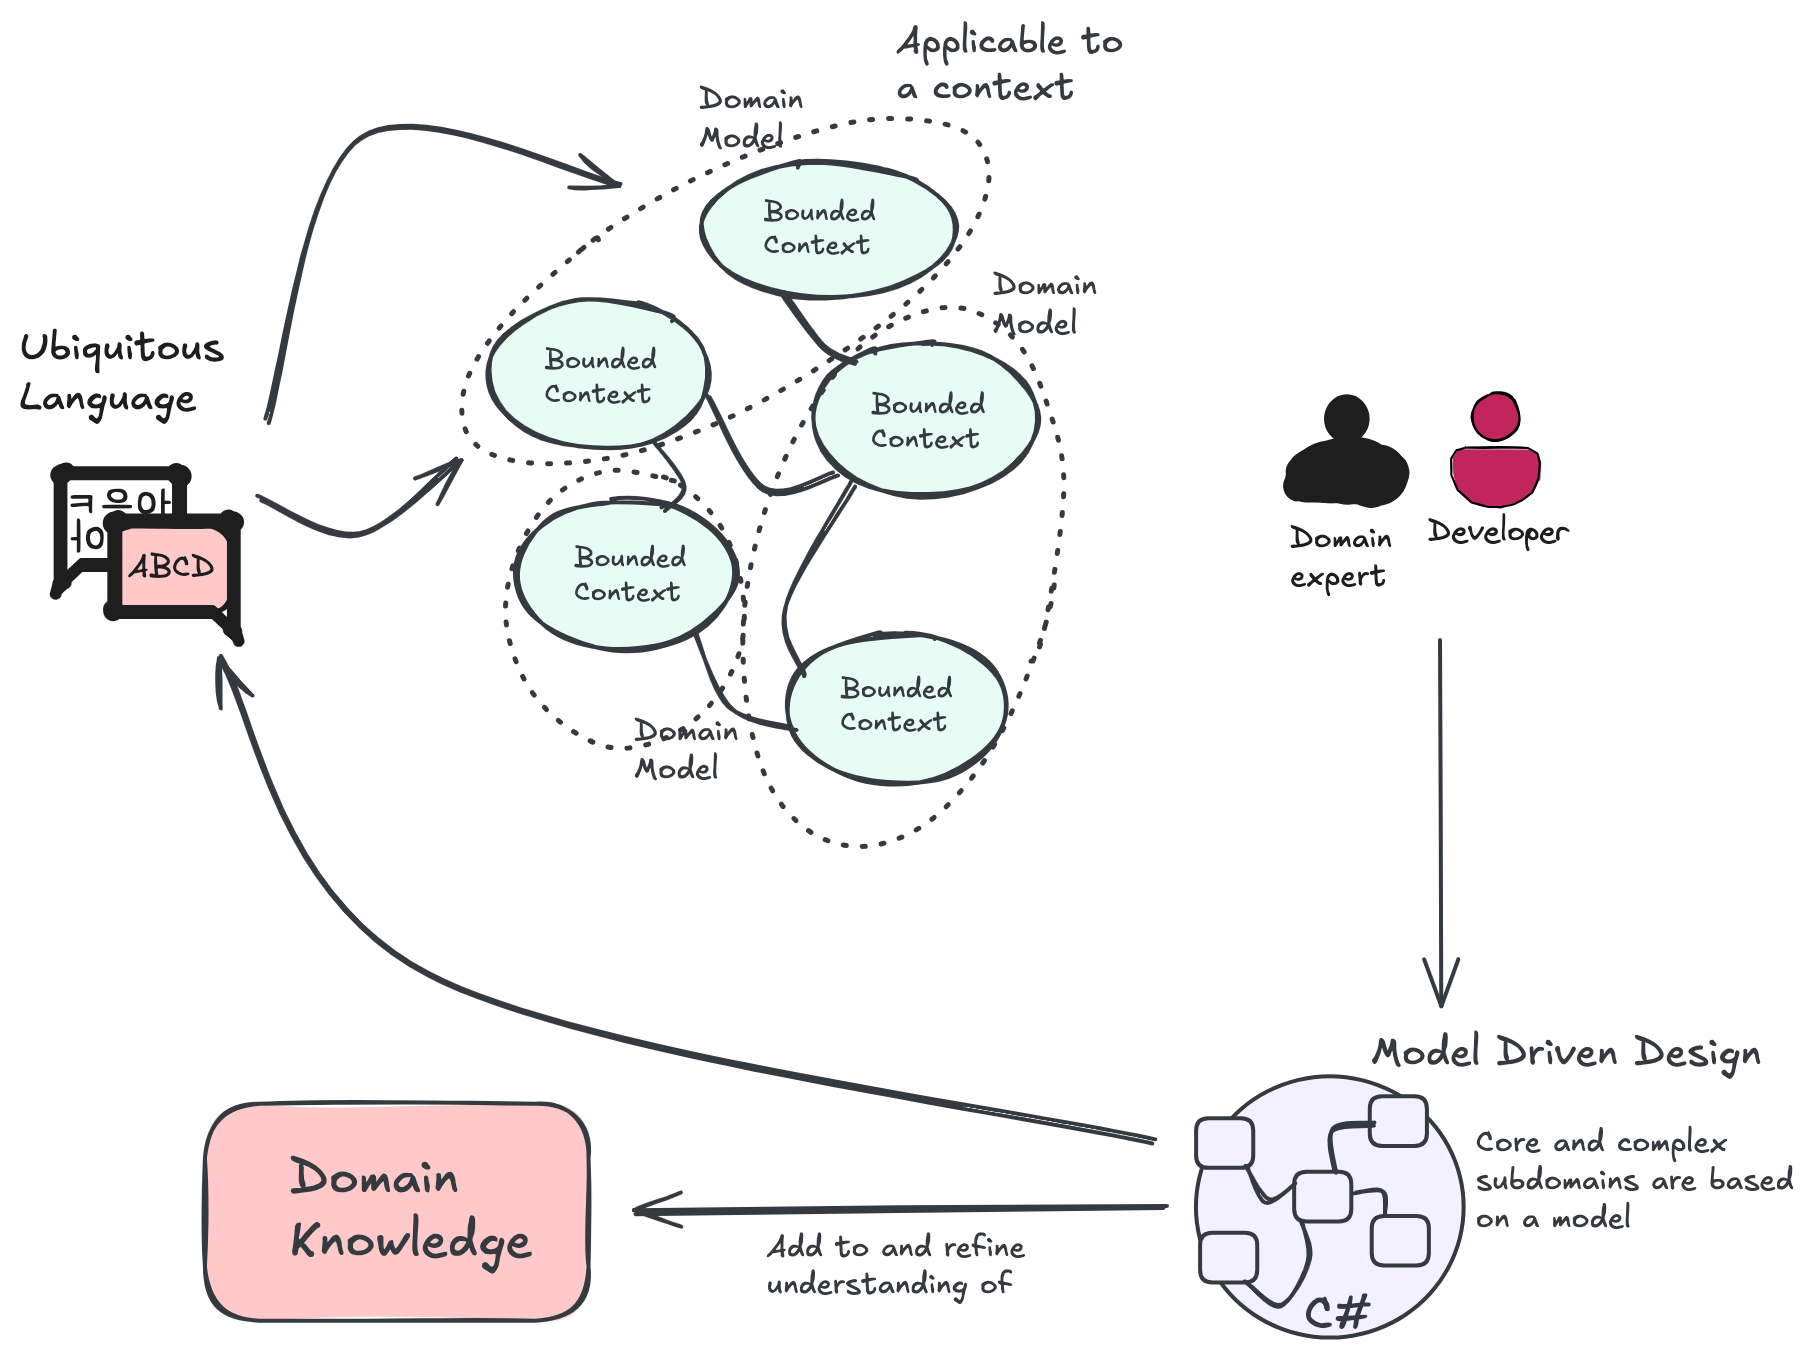
\includegraphics[width=0.8\linewidth]{BCS-Tessi//images/DDD_CicloSoftware.png}
            \caption[Come DDD permea il ciclo di vita del \textit{software}]{Come DDD permea il ciclo di vita di un \textit{software}.}
            \label{fig:DDD-generale}
        \end{figure}
        
        
        \noindent All'interno di SogeaSoft S.r.l., l'attività di sviluppo è organizzata mediante un sistema di \textit{task assignment}, in cui ogni attività (detta anche \textit{issue}) viene assegnata a uno sviluppatore specifico. Questo approccio favorisce un’elevata \textit{ownership} del lavoro, responsabilizzando il singolo sviluppatore e ottimizzando la gestione delle risorse.

        \vspace{0.2 em}
        \noindent A seconda del livello di urgenza e priorità, il Team Leader può collocare l’attività di implementazione all’interno del \textit{Backlog} specifico dello \textit{Sprint}, qualora si tratti di una lavorazione prioritaria, oppure nel \textit{Product Backlog}, in attesa di essere raffinata e pianificata nei successivi incontri di Raffinamento del \textit{backlog}.

        \vspace{0.2 em}
        \noindent Lo sviluppo del codice avviene secondo una strategia di \textit{Version Control} strutturata: per ogni attività assegnata, viene creato un \textit{branch} dedicato a partire dal ramo di sviluppo principale (develop). Tale \textit{branch} viene nominato seguendo una convenzione specifica, includendo parole chiave come "\textit{$feature_G$}" (nuova funzionalità) o "\textit{$bug_G$-fix}" (correzione di errori), seguite da una breve descrizione dell’attività, al fine di garantire una chiara identificazione e tracciabilità delle modifiche.

        \vspace{0.2 em}
        \noindent Una volta completata la fase di codifica, il codice prodotto è sottoposto a un processo di Verifica e Validazione (Sezione 1.6.4), il quale si concretizza nell'apertura di una \textit{Pull $Request_G$} ($PR_G$). Tramite la PR, lo sviluppatore richiede una revisione formale delle modifiche da parte del \textit{Team Leader} o di un altro membro del \textit{team} con pari competenze. Solo a seguito della validazione, il codice viene integrato nella \textit{codebase} principale attraverso un'operazione di \textit{merge} nel \textit{repository} del progetto, garantendo così il mantenimento della qualità del \textit{software} e la coerenza dell’intero sistema.

        
        \subsection{Verifica e Validazione}
        Il processo di Verifica ha l’obiettivo di fornire evidenza oggettiva della capacità del \textit{software} di soddisfare i requisiti e le caratteristiche definite.\footnote{ISO/IEC/IEEE 12207:2008 Software Verification Process, par 7.2.4.} Durante il mio periodo di \textit{stage}, ho avuto l'opportunità di assistere da vicino all'esecuzione delle attività legate a questo processo.

        \vspace{0.2 em}
        \noindent La verifica del \textit{software} si svolge in più fasi, partendo dalle singole unità di codice fino ad estendersi al sistema nel suo complesso. Le principali tipologie di \textit{test} utilizzate sono le seguenti:
        \begin{itemize}
        \item \textbf{\textit{Test} di unità}: verificano le singole unità di codice, ovvero porzioni atomiche ed eseguibili che espongono un comportamento specifico. Nello specifico ho avuto occasione di sviluppare \textit{test} specifici, progettati per verificare il soddisfacimento dei requisiti identificati;

        \item \textbf{\textit{Test} di integrazione}: questi \textit{test} verificano il comportamento e l'interazione tra le diverse parti del sistema, assicurandosi che il \textit{software} rispetti i requisiti funzionali previsti;

        \item \textbf{\textit{Test} di sistema}: questi test mirano a verificare la conformità del \textit{software} nel suo insieme, considerando le dipendenze tra le varie componenti.
        \end{itemize}

        \noindent In generale SogeaSoft S.r.l. adotta un processo di Verifica strutturato, seppur con una metodologia flessibile. La scrittura di \textit{test} non è obbligatoria per la presentazione e la validazione del \textit{software}. Tuttavia, quando presenti, i test vengono sviluppati direttamente all’interno dell'ambiente Microsoft Azure, sfruttando le sue \textit{$pipeline_G$}. In questo ambiente, il codice viene compilato e i \textit{test} vengono eseguiti automaticamente. Questi test vengono eseguiti sulle \textit{Pull Requests} (PR) nei \textit{branch} designati, garantendo che le modifiche apportate non introducano errori nel sistema. 

        \vspace{0.2 em}
        \noindent Il processo di Validazione invece fornisce evidenza oggettiva sulla capacità del \textit{software} di soddisfare le aspettative e i bisogni del committente.\footnote{ISO/IEC/IEEE 12207:2008 Software Validation Process, par 7.2.5.}

        \vspace{0.2 em}
        \noindent In SogeaSoft S.r.l. la validazione delle PR è un processo collaborativo che coinvolge più sviluppatori: i colleghi svolgono una revisione del codice e, salvo casi particolari, la validazione richiede l’approvazione di due revisori che non siano gli sviluppatori stessi delle modifiche. Inoltre, secondo il principio del \textit{Domain-Driven Design} (DDD), la validazione dovrebbe coinvolgere anche il \textit{domain expert}, poiché è colui che possiede una conoscenza approfondita del dominio applicativo e rappresenta il principale fruitore del servizio.

        \vspace{0.2 em}
        \noindent Nello specifico, la validazione dei risultati delle attività da me svolte è avvenuta attraverso incontri dedicati, in cui il lavoro completato è stato presentato e discusso con l'intero \textit{team}, durante due \textit{Sprint Review}. Questo approccio ha consentito non solo di rendere visibile a tutti, inclusi il \textit{Product Owner} e i membri del \textit{team} di sviluppo, il progresso e la qualità del lavoro, ma anche di allineare le attività agli obiettivi e ai requisiti stabiliti. Inoltre, tali incontri hanno offerto l'opportunità di identificare e risolvere eventuali problematiche emerse, assicurando che il progetto proseguisse in maniera coerente e conforme alle aspettative degli \textit{stakeholder}.
        
        \subsection{Manutenzione}
        Lo scopo del processo di Manutenzione del \textit{software} è fornire un supporto a un prodotto \textit{software} già consegnato. Questo processo include una serie di attività destinate a mantenere il software operativo e adeguato alle esigenze in continua evoluzione degli utenti e dell'ambiente. L'obiettivo principale è assicurare che il prodotto mantenga la sua funzionalità, affidabilità e performance nel tempo, minimizzando i costi associati dal momento della distribuzione fino al suo ritiro.\footnote{ISO/IEC/IEEE 12207:2008, Software Maintenance Process, par 6.4.10.}

        \vspace{0.2 em}
        \noindent Il \textit{Domain-Driven Design} (DDD) permea anche questa fase del ciclo di vita del \textit{software}. Dopo la messa in produzione, il modello di dominio potrebbe evolversi in risposta all'emergere di nuove esigenze o informazioni. Grazie alla natura iterativa e incrementale di DDD, il modello di dominio può essere continuamente aggiornato e migliorato attraverso il \textit{feedback} degli utenti o la scoperta di nuove dimensioni del dominio, attuando una manutenzione adattiva. Inoltre, DDD facilita l'adattamento ai cambiamenti delle esigenze aziendali, mantenendo il sistema allineato con gli obiettivi del \textit{business}, applicando una manutenzione preventiva. Durante la fase di manutenzione, è possibile rivedere i \textit{Bounded Contexts} e le comunicazioni tra i modelli di dominio, migliorando così la separazione delle preoccupazioni e garantendo che il \textit{software} continui a rispondere in modo adeguato alle evoluzioni del contesto operativo e strategico. Tale processo è rappresentato nel suo insieme nella Figura 1.9 nella pagina successiva:

        \begin{figure}[H]
            \centering
            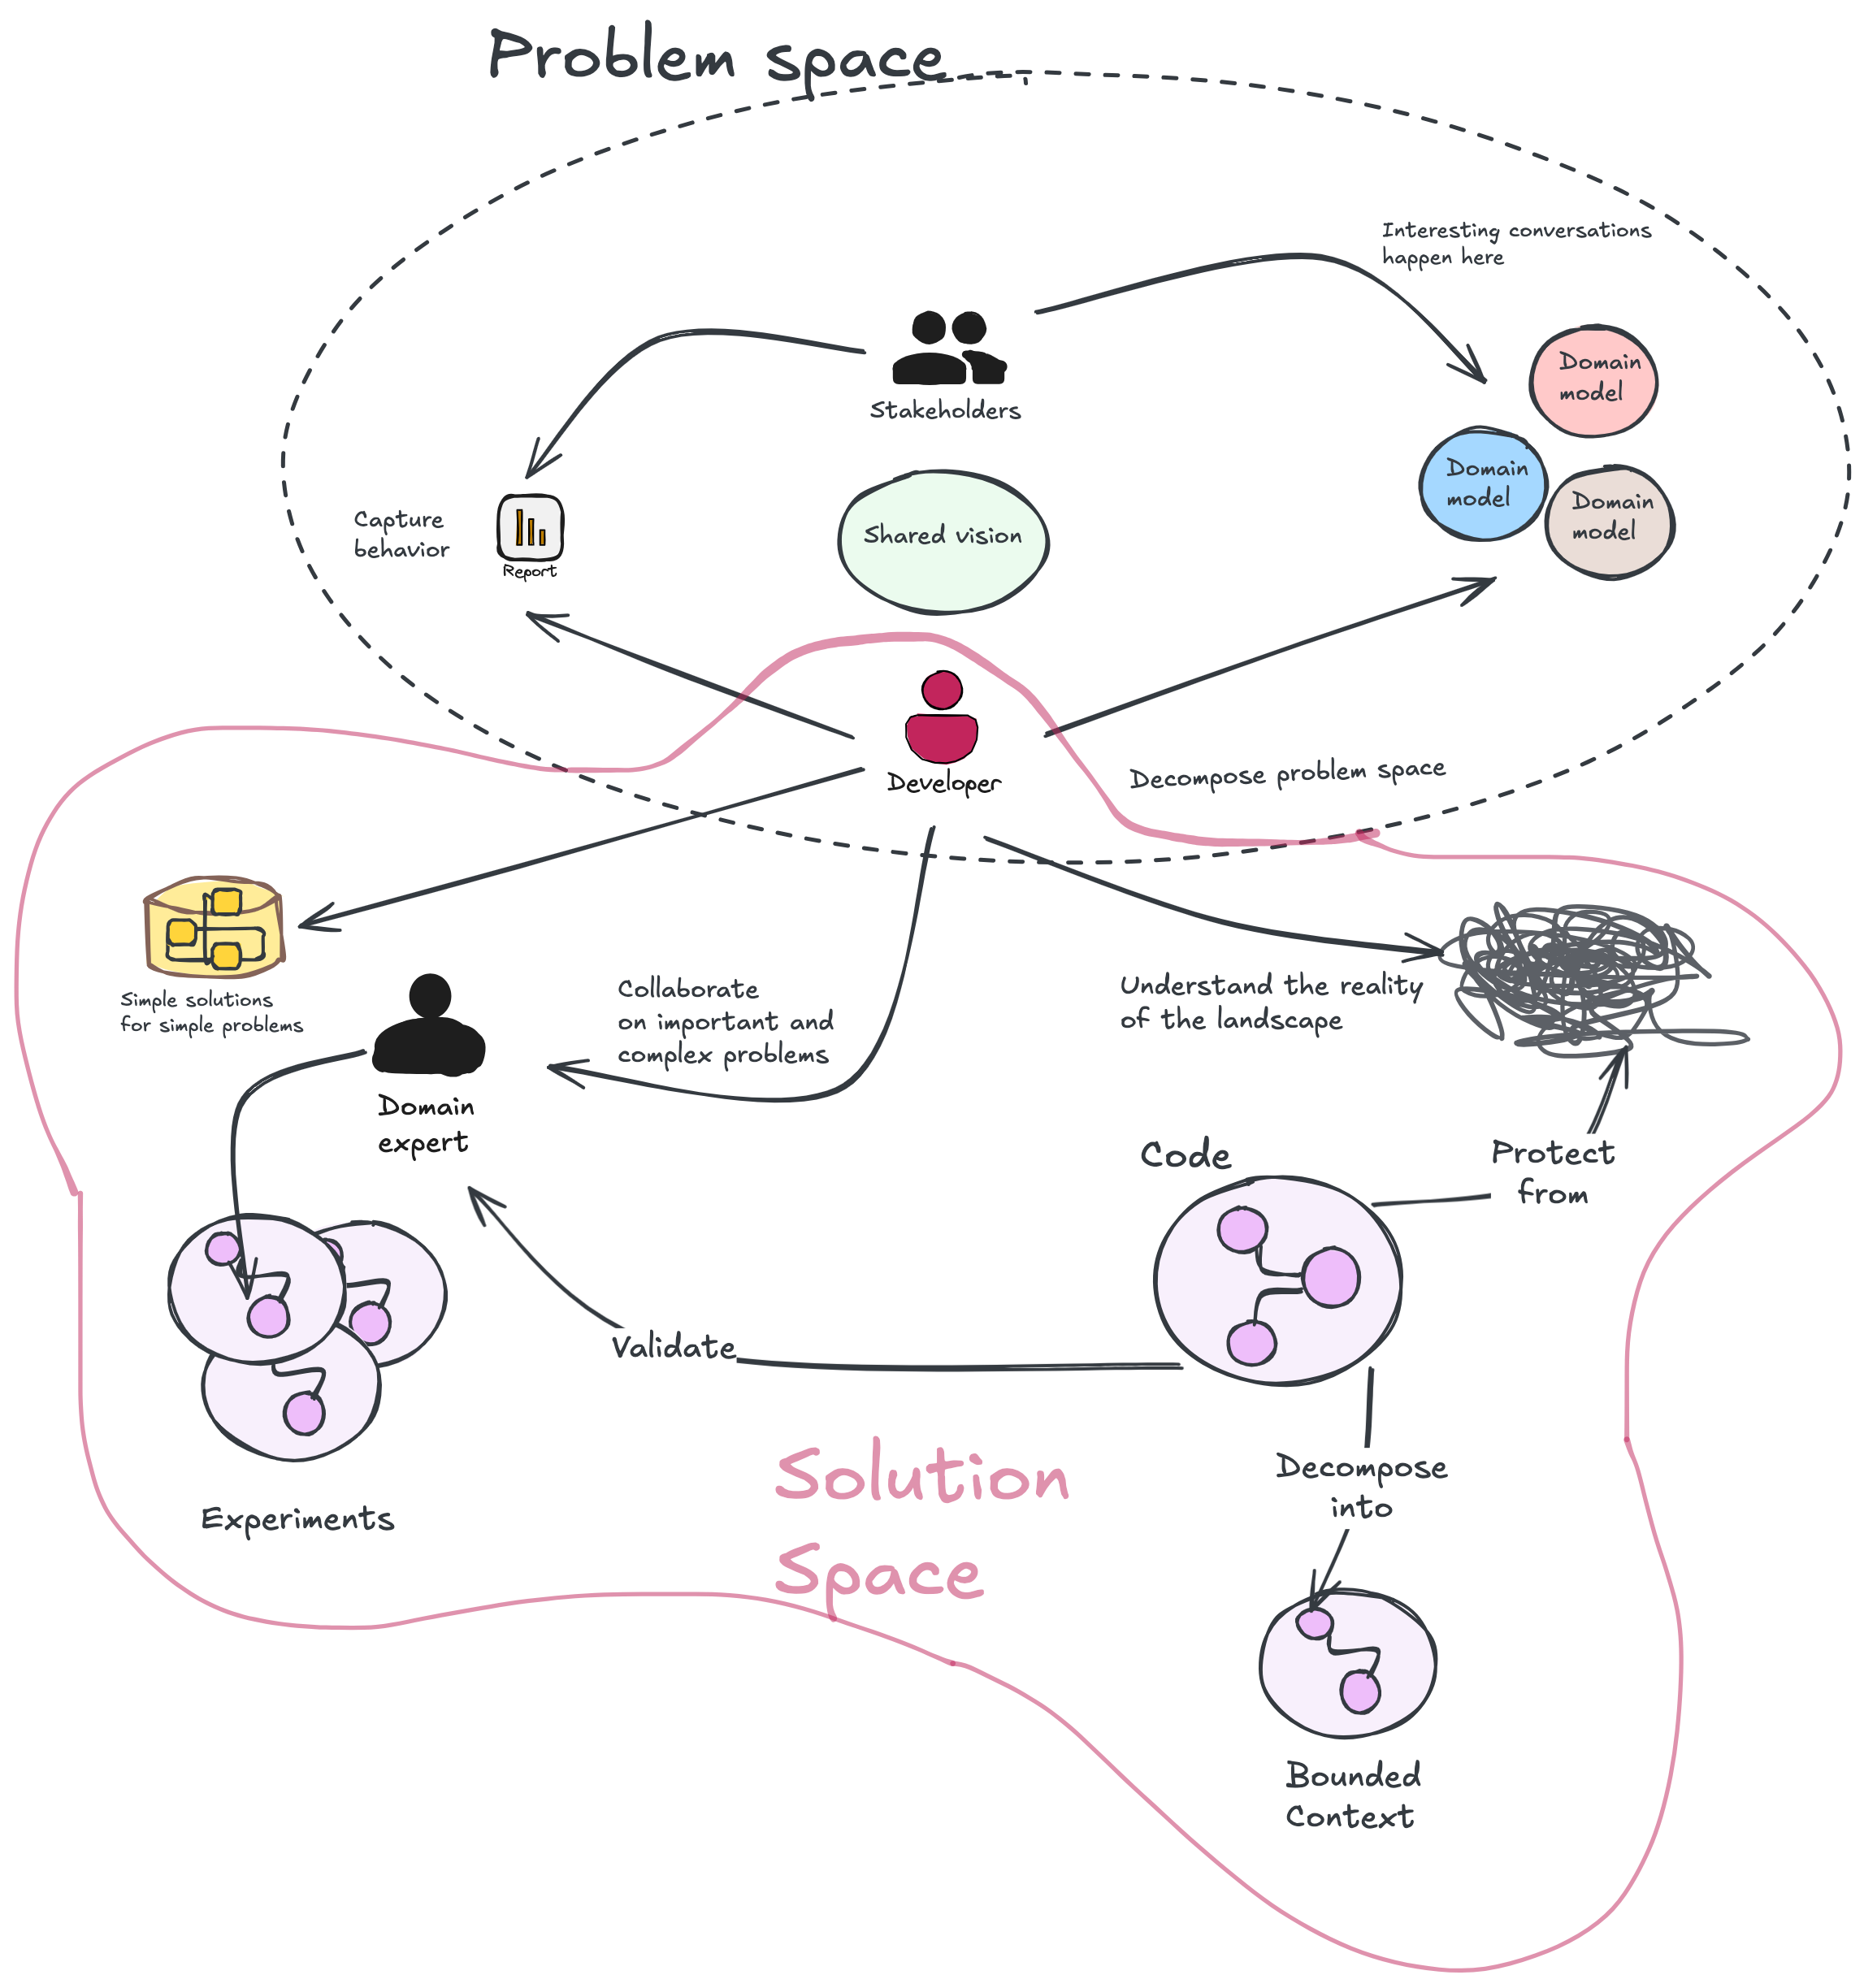
\includegraphics[width=0.8\linewidth]{BCS-Tessi/images/DDD_generale.png}
            \caption{Visione d'insieme dell'utilizzo di DDD nello sviluppo \textit{software}.}
            \label{fig:DDD-riassunto}
        \end{figure}

        
    \section{Tecnologie utilizzate}
    
    Per la realizzazione dei propri prodotti, SogeaSoft S.r.l. adotta un insieme di tecnologie predefinito e condiviso tra tutti i \textit{software} sviluppati. Tuttavia, tali tecnologie si sono progressivamente evolute per garantire l’aggiornamento rispetto agli sviluppi del settore. L’obiettivo dell’azienda è implementare un’architettura $esagonale_G$ nello sviluppo del \textit{software} SAI e delle sue declinazioni, ossia un modello di progettazione che consente la sostituzione o l’aggiornamento delle tecnologie senza alterare il comportamento del sistema sottostante, che rimane tecnologicamente agnostico.  

    \vspace{0.2 em}
    \noindent Come si può osservare in Figura 1.10, durante il mio \textit{stage}, una parte del processo di formazione (Sezione 1.5.3) è stata dedicata allo studio dell’evoluzione del sistema SAI, dal suo primo rilascio fino ad oggi, al fine di comprendere in modo più approfondito gli obiettivi del mio progetto. L’analisi delle tecnologie adottate in passato è rilevante perché una parte del progetto prevede l’aggiornamento del sistema tramite l’implementazione di soluzioni tecnologiche più moderne, garantendone la continuità operativa e l’efficienza.

    \vspace{0.2 em}
    \noindent I linguaggi di programmazione utilizzati sono:
    \begin{itemize}
        \item \textbf{C++}: è un linguaggio di programmazione orientato agli oggetti molto diffuso. In questo caso, è particolarmente apprezzato per la sua efficienza nell'elaborazione di operazioni ad alte prestazioni, la gestione diretta della memoria e la capacità di sviluppare applicazioni di sistema complesse. È alla base di tutto il sistema SAI;
        \item \textbf{C\#}: è un linguaggio orientato agli oggetti sviluppato da Microsoft, progettato per la creazione di applicazioni su piattaforme come Windows, \textit{web} e dispositivi mobili. È utilizzato in SAIonWeb, oggetto del mio progetto di \textit{stage}.
    \end{itemize}
    Questi linguaggi di programmazione sono utilizzati specificamente per lo sviluppo delle applicazioni basate sulla piattaforma SAI, mentre le tecnologie di supporto, che forniscono il fondamento per il funzionamento e la gestione del prodotto, comprendono una serie di strumenti e \textit{framework} integrati. Tali tecnologie sono:

    \begin{itemize}
        \item \textbf{Qt}: \textit{framework} multipiattaforma utilizzato principalmente per lo sviluppo di applicazioni con interfaccia grafica, alla base del sistema SAI.
        \item \textbf{KDE}: è un ambiente \textit{desktop} \textit{open-source} per sistemi operativi Linux. Offre un'interfaccia grafica altamente personalizzabile, con un focus sull'usabilità e sull'integrazione di applicazioni. Il suo \textit{framework} di sviluppo è Qt .
        \item \textbf{Angular}: è un \textit{framework} \textit{open-source} per lo sviluppo di \textit{single-page web $application_G$} ($SPA_G$) ossia siti \textit{web} composti da una sola pagina che aggiorna dinamicamente il contenuto senza ricaricare l'intera pagina. Con il suo approccio basato su componenti, Angular promuove lo sviluppo modulare e scalabile, motivo per cui è stato scelto da SogeaSoft S.r.l. in SAIonWeb. 
        \item \textbf{ASP.NET Core}: è un \textit{framework} \textit{open-source} per lo sviluppo di applicazioni \textit{web} moderne e scalabili. Permette di creare applicazioni \textit{web}, $API_G$ e microservizi, supportando C\#.
    \end{itemize}

    \begin{figure}[H]
        \centering
        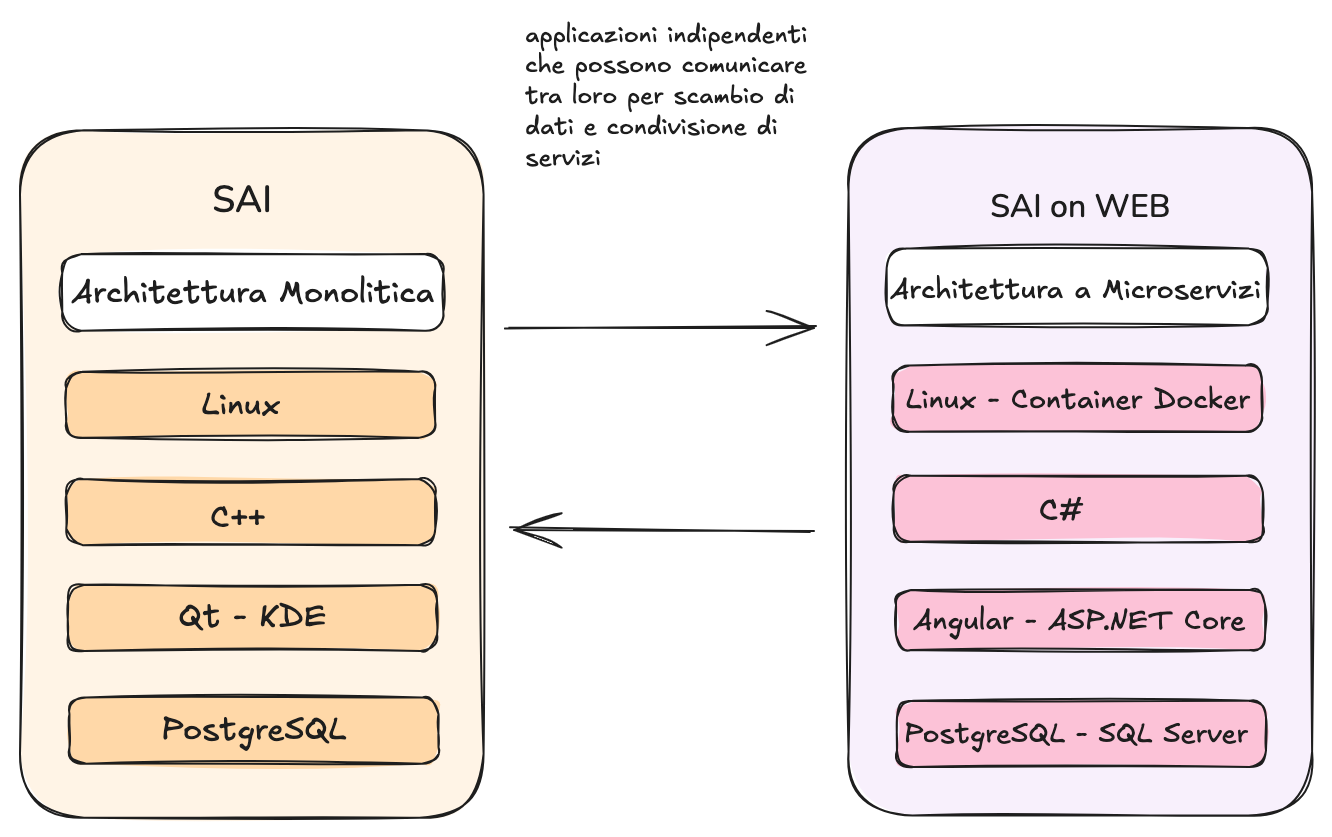
\includegraphics[width=0.8\linewidth]{BCS-Tessi/images/SAI_microservizi.png}
        \caption[Tecnologie utilizzate in SogeaSoft S.r.l.]{Schema delle tecnologie utilizzate da SogeaSoft S.r.l. Informazioni apprese durante il processo di formazione}
        \label{fig:Tecnologie}
    \end{figure}

    \noindent L'ambiente di sviluppo in SogeaSoft S.r.l. è configurato per operare principalmente su sistemi basati su Linux o, in alternativa, su \textit{container} $Docker_G$ eseguiti su sistemi operativi Windows. Questo approccio consente una maggiore flessibilità e compatibilità con diverse configurazioni di sistema. Il processo di codifica si svolge localmente sulle singole \textit{workstation}, dove gli sviluppatori utilizzano Microsoft Visual Studio, un ambiente di sviluppo integrato (IDE) altamente configurabile e supportato.

    \vspace{0.2 em}
    \noindent Il tracciamento delle modifiche apportate al codice secondo il controllo di versione avviene con l'uso di $Git_G$, un particolare \textit{Version Control System} (VCS). 

    \vspace{0.2 em}
    \noindent 
    SAI è il \textit{framework} di base su cui si fondano tutti i prodotti derivati di SogeaSoft S.r.l. Si tratta di un sistema piuttosto datato, che utilizza tecnologie oggi difficili da manutenere, da cui nasce la necessità di migrare verso un'architettura a microservizi. La logica sottostante risulta complessa da modificare, pertanto sono state adottate diverse soluzioni. Ad esempio, il sistema impiega un'architettura basata su \textit{web service}, che adotta il modello \textit{Representational State $Transfer_G$} ($REST_G$) per lo scambio di dati tra i moduli. Questo modello architetturale prevede che le informazioni transitino tramite connessioni dedicate, note come \textit{Application Programming $Interfaces_G$} ($API_G$). Tuttavia, tale modello non definisce l'intero sistema, poiché la fase di migrazione è ancora in corso e rappresenta il \textit{focus} principale del mio progetto di \textit{stage}, come verrà approfondito nella Sezione 2.
    
    \vspace{1em}
    
    \noindent Nel dettaglio si utilizzano:
    \begin{itemize}
        \item \textbf{Advanced Message Queuing $\textbf{Protocol}_G $($\textbf{AMQP}_G$)}:  è un protocollo di messaggistica \textit{open-source} progettato per la gestione affidabile e sicura delle code di messaggi tra sistemi distribuiti. È utilizzato da SogeaSoft S.r.l. per facilitare l'integrazione tra le applicazioni e la gestione dei flussi di dati.
        
        \item \textbf{RabbitMQ}: è un \textit{$Message Broker_G$} \textit{open-source} che implementa il protocollo AMQP per la gestione di code di messaggi tra applicazioni. Permette una comunicazione asincrona e affidabile tra sistemi distribuiti.

        \item \textbf{Debezium}: è una piattaforma \textit{open-source} per il cambiamento di dati in tempo reale che consente di monitorare e registrare le modifiche apportate ai database. Essa si integra con sistemi di messaggistica come RabbitMQ per diffondere le modifiche ai dati attraverso flussi di eventi.
        
        \item \textbf{Swagger}: è uno strumento che fornisce un'interfaccia grafica interattiva per esplorare e testare le API RESTful. Permette agli sviluppatori di testare \textit{$endpoint_G$} API direttamente dal \textit{$browser_G$} senza bisogno di scrivere codice aggiuntivo.
        
        \item \textbf{DBeaver}: \textit{$client_G$} utilizzato per accedere, interrogare e manipolare \textit{database} relazionali basati sul \textit{Structured Query $Language_G$} ($SQL_G$), un linguaggio di manipolazione dei dati ampiamente diffuso.
    \end{itemize}

    \noindent Riguardo ai sistemi di gestione dei \textit{database}, SogeaSoft S.r.l. supporta una varietà di \textit{Database Management $Systems_G$} ($DBMS_G$), offrendo così una notevole flessibilità nella gestione e nell'archiviazione dei dati. Durante il mio \textit{stage}, ho avuto l'opportunità di interagire con diversi DBSM, tra cui PostgreSQL, SQL Server e IBM DB2, che sono tra le soluzioni più comunemente utilizzate dalle aziende clienti.
    
    
    \section{L’innovazione in SogeaSoft}

    Le informazioni sulle innovazioni tecnologiche adottate da SogeaSoft S.r.l. mi sono state fornite principalmente tramite i racconti del mio \textit{tutor}, che ha condiviso con me le pratiche aziendali e i progetti più recenti. Non essendo disponibili dati documentati diretti o misurazioni quantitative, mi sono basata sulla descrizione dei processi e delle soluzioni adottate durante il mio periodo di \textit{stage}.

    \vspace{0.2 em}
    \noindent Sebbene l'azienda non abbia intrapreso l'adozione di innovazioni radicali, la sua capacità di evolversi in modo continuo e sostenibile le ha consentito di mantenere una posizione competitiva nel mercato. L'approccio adottato, che prevede l'allocazione di risorse umane e finanziarie in base alle necessità percepite, ha favorito l'implementazione di miglioramenti incrementali, garantendo così una continua crescita della capacità produttiva e un aggiornamento regolare delle tecnologie impiegate.
    
    \vspace{0.2 em}
    \noindent Tuttavia, SogeaSoft S.r.l. ha considerato la migrazione verso un'architettura a microservizi solo quando il processo di manutenzione del \textit{software} (Sezione 1.6.5) è diventato eccessivamente oneroso. Questo è avvenuto a causa della crescente difficoltà di gestire le tecnologie obsolete, che richiedevano modifiche strutturali complete del sistema, una soluzione che si è rivelata non praticabile nel lungo periodo. 

    \vspace{0.2 em}
    \noindent Una volta che l'azienda ha riconosciuto l'importanza di integrare nuove tecnologie pur mantenendo intatto il sistema di base, si è manifestato un crescente interesse per l'innovazione. Ad esempio, durante il mio \textit{stage}, ho avuto l'opportunità di implementare una \textit{demonstration} utilizzando la tecnologia RabbitMQ (approfondita nella Sezione 1.7), in cui ho sviluppato un sistema di aggiornamento dei dati in tempo reale. Questa \textit{demo} ha comportato l'impiego di tecnologie relativamente recenti e, nel caso di Debezium (Sezione 1.7), non ufficialmente documentate per questa combinazione specifica\footnote{Fonte: \href{https://debezium.io/documentation/reference/3.1/connectors/index.html}{Documentazione ufficiale di Debezium, Source Connectors.}}. 

